\documentclass[letterpaper,11pt] {article}

%---------------------------------------------------------------------------
%---------------------PAQUETES UTILIZADOS (CON EXPLICACIÓN) ----------------
%---------------------------------------------------------------------------

%-----------------------PRESENTACIÓN Y FORMATO -----------------------------
%\usepackage{pslatex}	%----------USO DE TIMES NEW ROMAN -------------
\usepackage{graphicx}
\usepackage{wrapfig}
\usepackage{multicol}
\usepackage{multirow}
\usepackage[margin=2cm]{geometry}
\usepackage[export]{adjustbox}
\usepackage[labelfont=bf,font=scriptsize, margin=10pt]{caption}
\usepackage[labelformat= simple]{subcaption}
			\renewcommand*{\thesubfigure}{\alph{subfigure})}
\usepackage{mathtools}
\usepackage{physics}

\setlength{\parskip}{1em}
\setlength{\parindent}{3em}
\usepackage[bottom]{footmisc}
%--------------------------------------------
\usepackage{xcolor} 
	\definecolor{bone}{RGB}{253,255,224}  %hueso
	\definecolor{lgreen}{RGB}{146,197,130} %light green,
	\definecolor{lblue}{RGB}{134,165,169} %light blue
	\definecolor{lgray}{RGB}{118,118,118} %light gray
	\definecolor{dgreen}{RGB}{83,111,80}%dark green
\usepackage[colorlinks, 
			linkcolor=lblue,
			citecolor=lgreen]{hyperref}

%-----------------------IDIOMA Y BIBLIOGRAFÍA -- ----------------------------
\usepackage[spanish, es-tabla]{babel} %------ ESPAÑOL (TABLA) ----------
\usepackage[T1]{fontenc}			  %-------- 8-BITS FONT ------------
\usepackage[utf8]{inputenc}           %------- ALFABETO ----------------
\spanishdecimal{. }
\usepackage[numbers,sort&compress]{natbib}


%------------------------- MATEMÁTICAS --------------------------------------
\usepackage{amsmath}
\usepackage{mathrsfs}
\usepackage{amssymb}
\usepackage{empheq}
\usepackage[most]{tcolorbox}
\tcbset{colback=green!60!blue, colframe= green!50!blue,
		  colbacktitle = green!50!blue, sharp corners = downhill, 
		  fonttitle=\bfseries, leftrule = 5mm}

	\newcommand{\beqhalf}{\noindent \begin{minipage}[c]{. 5\linewidth} \begin{equation}}
	\newcommand{\eeqhalf}{\end{equation} \end{minipage} }
	\newcommand{\eqhalf}[1]{\beqhalf #1 \eeqhalf}	


%--------------------- IMAGENES ---------------------------------------------
\graphicspath {{0-Images/}}
\usepackage{tikz,pgfplots}
\usetikzlibrary{decorations.shapes}
\usetikzlibrary{arrows.meta,calc,decorations.markings,math,arrows.meta}
\usetikzlibrary{%
    decorations.pathreplacing,%
    decorations.pathmorphing%
}
\usepackage{tikz-3dplot}

%---------------------  DATOS DEL ESCRITO ------------------------------------
\title{Reflectancia de sistemas monocapa con nanopartículas esféricas metálicas  usando el modelo de esparcimiento coherente }
\author{Jonathan Alexis Urrutia Anguiano}
\date{}

%---------------------  INICIO DEL TEXTO ------------------------------------
\begin{document}\maketitle

Las propiedades f\'isicas de los materiales dependen en general del tamaño del sistema \cite{boverhof2015comparative}, por ejemplo, a escala nanom\'etrica ---de $1$ a $100$ nm \cite{boverhof2015comparative}---, la respuesta electromagn\'etica (EM) de bulto de los metales es menos relevante que los efectos de superficie \cite{zhao2008methods}.  La \emph{nanoplasm\'onica} estudia la respuesta EM a esta escala y el inter\'es en su estudio se ha renovado debido a las posibles aplicaciones que emplean las resonancias plasm\'onicas de superficie (SPRs).  Áreas como la espectroscop\'ia \cite{novotny2006principles}, el sensado \cite{jain2008noble}, la litograf\'ia \cite{stockman2011nanoplasmonics}, y la biolog\'ia y  medicina \cite{jain2008noble}, son ejemplos del creciente interés en la nanoplasmónica. 

Los plasmones son oscilaciones colectivas de los electrones en un material metálico,  resultado del  acoplamiento con la radiaci\'on EM a las frecuencias donde ocurren las SPRs \cite{stockman2011nanoplasmonics}.  La clasificación de los plasmones comprende  dos tipos: propagantes y localizados.  Cuando los plasmones se propagan a lo largo de una interfaz plana entre un medio diel\'ectrico y uno met\'alico se denomina  \emph{plasm\'on-polarit\'on de superficie} (SPP) \cite{maier2007plasmonics}.  Si el plasmón, en cambio, se encuentra en la superficie de una partícula  met\'alica, de tamaño finito, se le conoce como \emph{resonancia de plasm\'on de superficie localizado} (LSPR) \cite{maier2007plasmonics}. 

%%%%%%%%%%%%%%%%%%%%%%%%%%%%%%%%%%%%%%%%%%%%%%%%%%%%%%%%%%%%%%%%%%%%%%%%%
%%%					WRAP FIGURE:
%%%					PRISMA EN ATR
%%%%%%%%%%%%%%%%%%%%%%%%%%%%%%%%%%%%%%%%%%%%%%%%%%%%%%%%%%%%%%%%%%%%%%%%%
\begin{wrapfigure}{h}{6.5cm}\centering
%	\begin{tikzpicture}[scale=.4]
%	\def\r{. 2}
%	\foreach \i in {-3. 5,-3,. . . ,3. 5}{
%		\fill[ball color=yellow,opacity = 1] (\i,2*\r) circle(\r);};
%	\fill[blue, opacity = . 5] (-4,0)--(4,0)--(0,-4);
%	\draw[- latex, red, thick](-2. 5,-4)--(-2,-2)--(0,0)--(2,-2)--(2. 5,-4) node[anchor = west]{\color{black}$\lambda$};
%	\draw[dashed, thick, gray](0,0)--(0,-4);
%	\path (0,-1. 25) node[anchor= west]{$\theta_i$} node[anchor=east] {$\theta_i$};
%	\end{tikzpicture}
	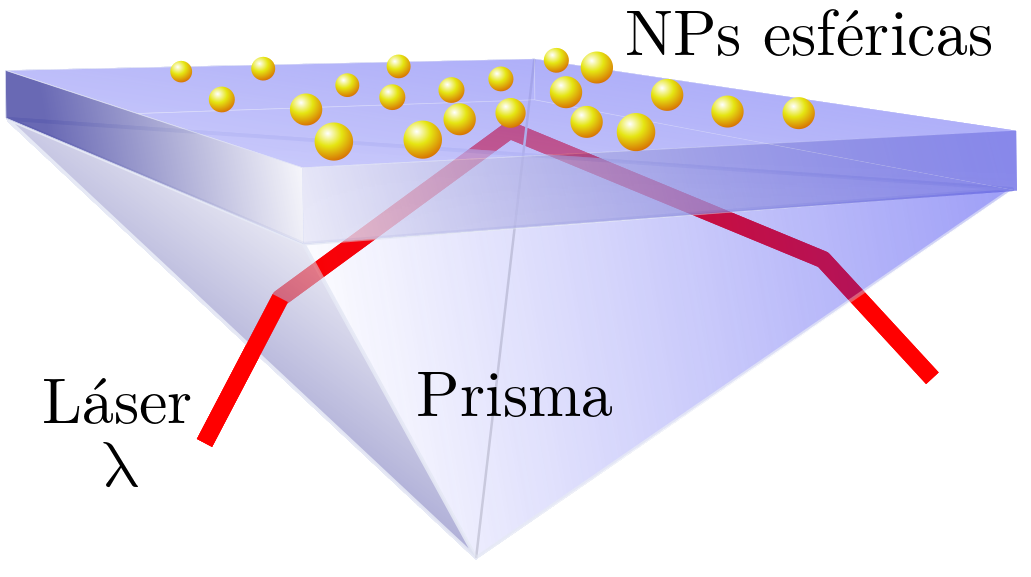
\includegraphics[scale=.18]{CSM_3D-Prism_Text.png}
	\caption{ Arreglo de NPs esf\'ericas iluminado por un haz de longitud de onda $\lambda$ a un \'angulo de incidencia $\theta_i$, en configuraci\'on ATR}
	\label{fig:ATR1}
\end{wrapfigure}
%%%%%%%%%%%%%%%%%%%%%%%%%%%%%%%%%%%%%%%%%%%%%%%%%%%%%%%%%%%%%%%%%%%%%%%%%
%%%					WRAP FIGURE:
%%%					PRISMA EN ATR
%%%%%%%%%%%%%%%%%%%%%%%%%%%%%%%%%%%%%%%%%%%%%%%%%%%%%%%%%%%%%%%%%%%%%%%%%

En el área de biosensores se emplean las SPRs por la respuesta que tienen ante cambios del índice de refracción de la matriz \cite{kabashin2009plasmonic}, que es el medio que rodea la estructura metálica.  Los sensores comerciales se caracterizan por el uso de SPPs en una configuración de incidencia interna atenuada (ATR), en donde el índice de refracción del medio donde incide la luz que ilumina a la estructura metálica es mayor al de la matriz (ver Fig.  \ref{fig:ATR1}).  Las mediciones de reflectancia, en un sistema en configuración ATR, presentan mínimos para determinadas combinaciones de  ángulos de incidencia $\theta_i$ y longitud de onda $\lambda$  \cite{danilov2018ultra}.  Los sensores basados en las LSPRs se han propuesto como mejora sobre los sensores comerciales, ya que estos son al menos un orden de magnitud más sensibles a cambios de índice de refracción de la matriz  que los sensores basados en SPPs \cite{jain2008noble,kabashin2009plasmonic}. 

\section{Antecedentes}

En el 2009 se public\'o un art\'iculo \cite{kabashin2009plasmonic} en el que se propone un sistema bidimensional de NPs cilíndricas de oro, colocadas en arreglos periódicos, para la mejora en resoluci\'on  del biosensado; las dimensiones de los nanocilindros y el parámetro de red del arreglo son menores que la longitud de onda con la que se ilumina el arreglo \cite{kabashin2009plasmonic}.  En el artículo se reportó un modo plasmónico distinto a los modos normales de las NPs individuales, que permite el sensado del índice de refracción de la matriz.  En el 2018 se publicó que este modo es una respuesta colectiva del arreglo periódico \cite{danilov2018ultra} y depende del parámetro de red.  

 En la Fig.  \ref{sfig:DipATR} se presentan los resultados de reflectancia en ATR, como función de la longitud de onda $\lambda$ para distintos ángulos de incidencia $\theta_i$, obtenidos mediante una simulación numérica para un arreglo cuadrado de nanocilindros, considerados como nanoesferoides, al emplear una modificación del modelo de Maxwell Garnett \cite{atkinson2006anisotropic} ---que es una teoría de medio efectivo\footnote{Proceso de homogenización en donde se sustituye el medio heterogéneo por un medio continuo equivalente.  Este proceso se basa en la respuesta promedio del medio original cuando la longitud de onda de la luz incidente es grande en comparación a las dimensiones del sistema \cite{sihvola1999mixing}. }--- para la función dieléctrica efectiva de la monocapa $\varepsilon(\omega) = n^2 (\omega)$.   En la Fig.  \ref{sfig:k(w)Kobashin} se grafica la relación de dispersión  (energía de la onda incidente como función de la  proyección perpendicular al sustrato del vector de onda) calculada numéricamente del arreglo simulado en la Fig.  \ref{sfig:DipATR}.  En la Fig.  \ref{sfig:PsiDelta} se grafican los resultados experimentales de los parámetros elipsométricos\footnote{$R_s/R_p = \tan\Psi e^{i\Delta}$, con $R_p$ la reflectancia en polarización \emph{p} y $R_s$ la reflectancia en polarización \emph{s} \cite{danilov2018ultra}. } $\Psi$ y $\Delta$ como función de $\lambda$ para un arreglo de NPs cilíndricas en un arreglo cuadrado y ordenado. 

	\begin{figure}[h!]\centering
		\begin{subfigure}{.01\linewidth}\caption{ }\label{sfig:DipATR} \vspace{3.5cm}	\end{subfigure}  
		\begin{subfigure}{.29\linewidth}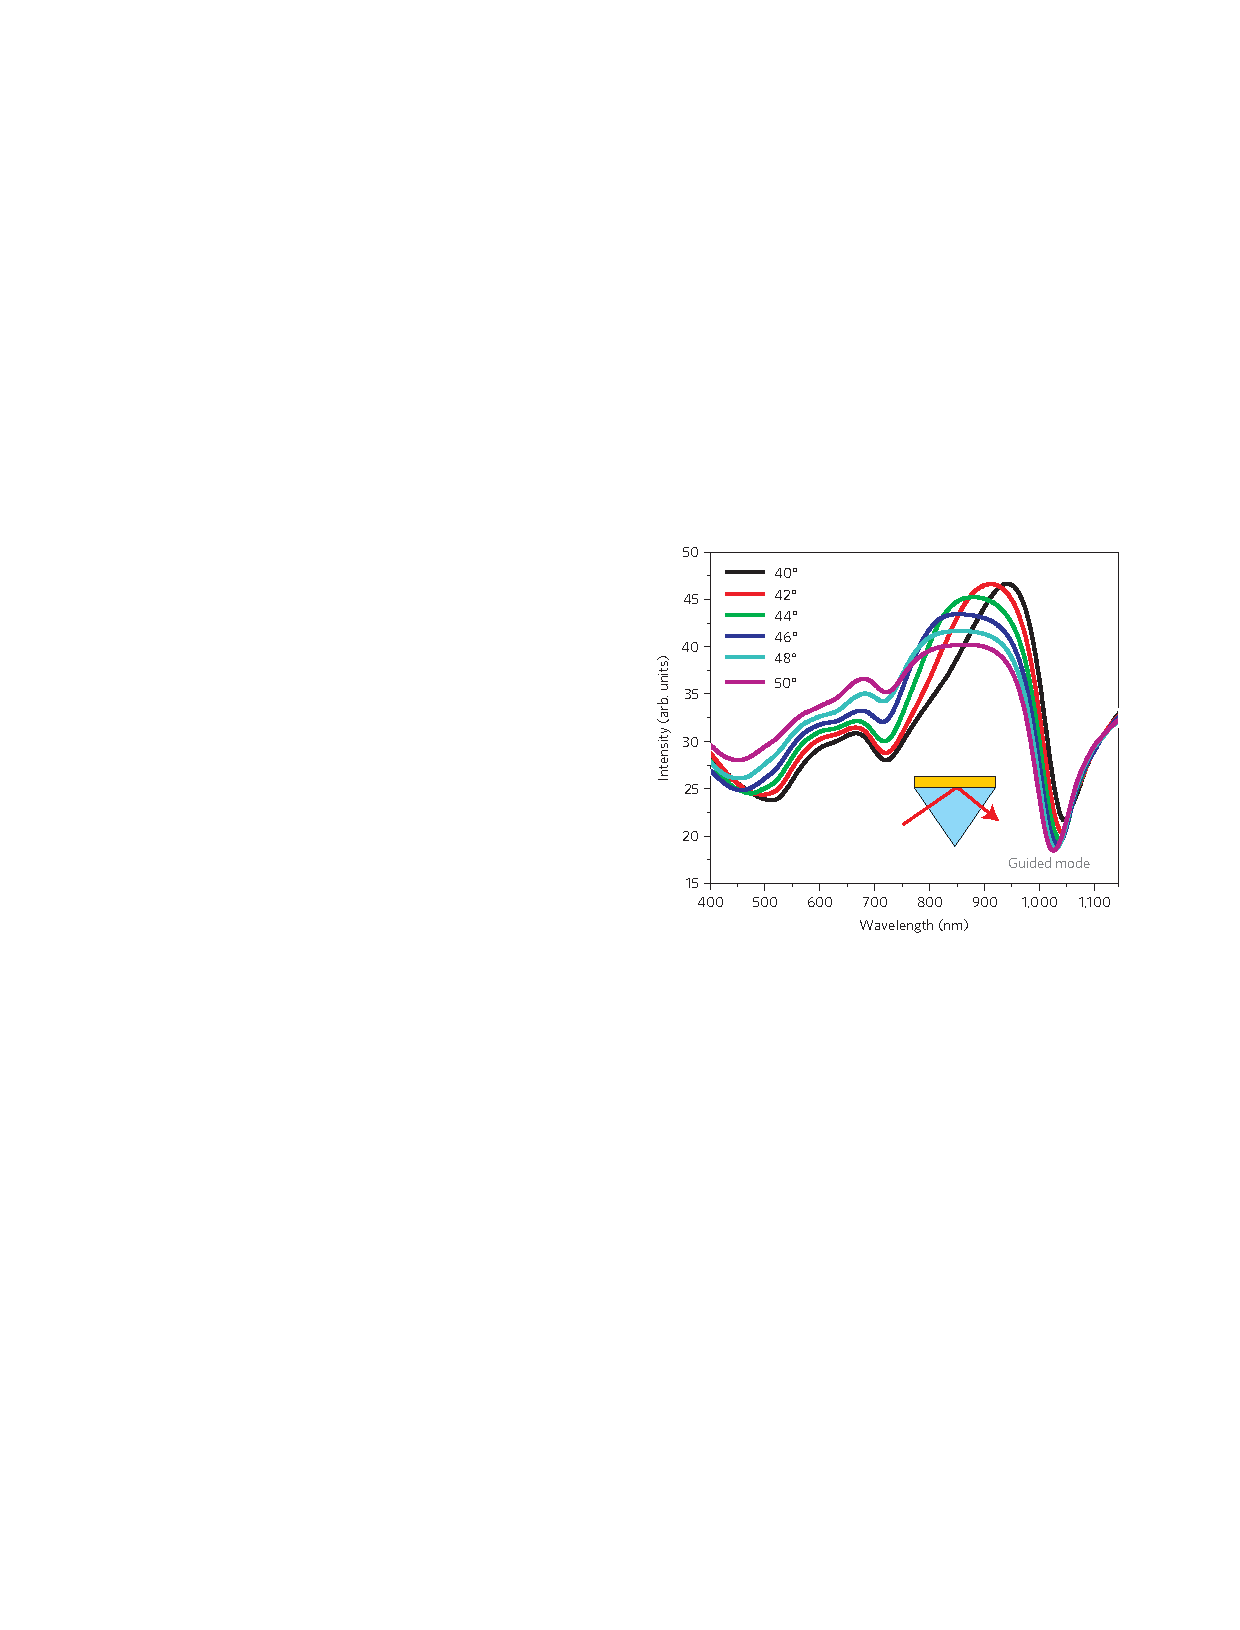
\includegraphics[scale=.68]{0-ATRKobashin2009}\end{subfigure}	\hspace{1em}
		\begin{subfigure}{.01\linewidth}\caption{ }\label{sfig:k(w)Kobashin} \vspace{3.5cm}	\end{subfigure} 
		\begin{subfigure}{.28\linewidth}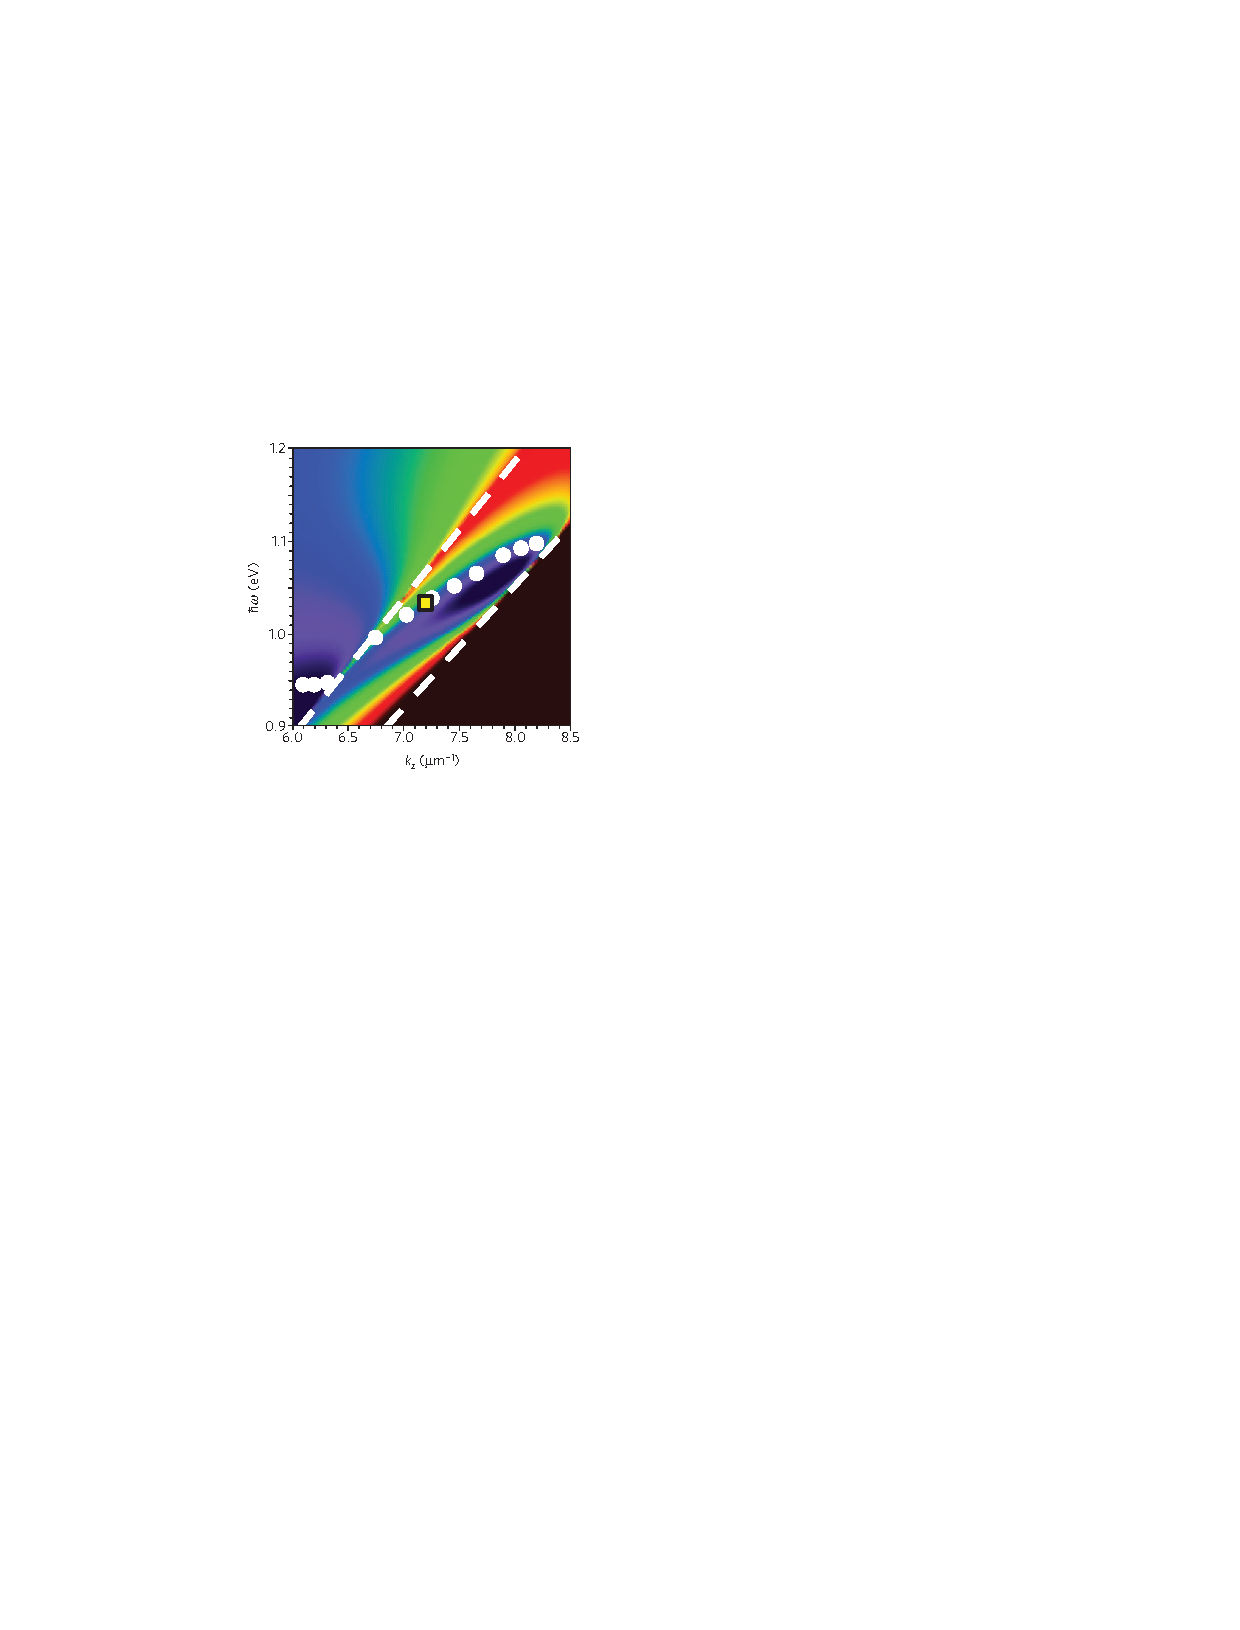
\includegraphics[scale=.81]{0-k(w)Kobashin2009}\end{subfigure}		
		\begin{subfigure}{.01\linewidth}\caption{ }\label{sfig:PsiDelta}\vspace{3.5cm}\end{subfigure}  
		\begin{subfigure}{.33\linewidth}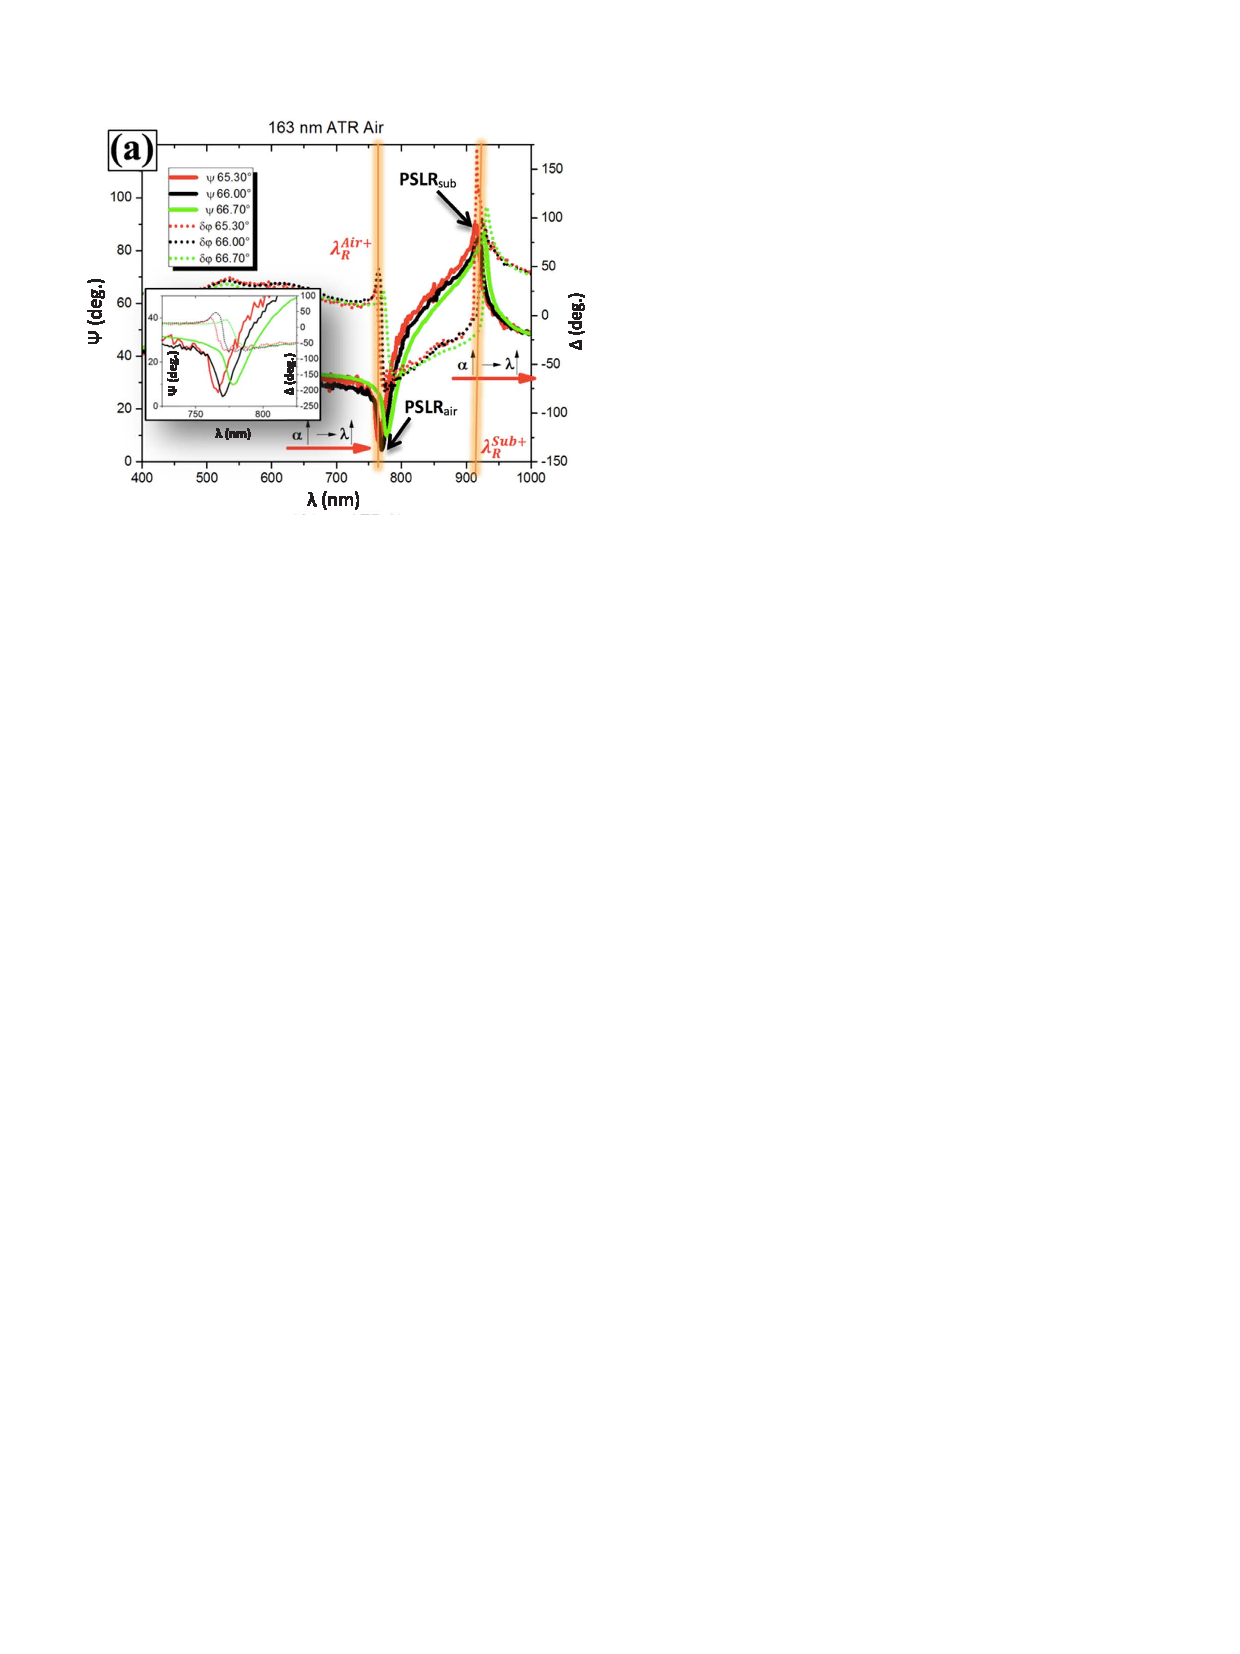
\includegraphics[scale=.7]{0-ATRSingleDanilov2018}\end{subfigure}
		\caption{\textbf{a)} Gráfica de la reflectancia  para un sistema periódico cuadrado de nanocilíndros de oro en ATR como función de la longitud de onda $\lambda$, para distintos ángulos de incidencia; y \textbf{b)} gráfica de la relación de dispersión  del arreglo  (extraídas de \cite{kabashin2009plasmonic}).  \textbf{c)} Gráfica de los parámetros elipsométricos (extraída de \cite{danilov2018ultra}) de un sistema de nanocilindros en un arreglo cuadrado periódico, en configuración ATR, en función de $\lambda$.  Las dimensiones de los nanocilindros en \textbf{a,b)} son $360$ nm de largo, $25$ nm de diámetro y una separación de $60$ nm entre ellos; los nanocilíndos están inmersos en una matriz de aire ($n=1$), sobre un sustrato de vidrio ($n=1. 5$).  Las dimensiones de los nanocilindros en \textbf{c)} son $163$ nm de largo, y un parámetro de red de $320$ nm; la matriz y el sustrado empleados son los mismos que en \textbf{a)} y \textbf{b)}. }\label{fig:GraphsPapers}
	\end{figure}
	
	
En la Fig.  \ref{sfig:DipATR}  se observan las resonancias plasmónicas típicas de NPs individuales (resonancia dipolar alrededor de $720$ nm y cuadrupolar alrededor de $500$ nm).  Adicionalmente, se observa una excitación a energía más baja que la del modo dipolar, por lo que no puede ser una resonancia de NP individual y por tanto debe corresponder a un modo colectivo, denominado \emph{modo guiado} en  \cite{kabashin2009plasmonic}.  El modo guiado se encuentra alrededor de los $1,000$ nm y sufre un corrimiento al azul conforme el ángulo de incidencia aumenta.  En la Fig.  \ref{sfig:k(w)Kobashin} se grafica la relación de dispersión del modo guiado, donde los puntos blancos corresponden a los mínimos en la reflectancia alrededor de los $1,000$ nm de la Fig.  \ref{sfig:DipATR} del modo guiado.  Las líneas punteadas en la Fig.   \ref{sfig:k(w)Kobashin} corresponden a los ángulos críticos de las interfaces del medio efectivo simulado con el aire (línea izquierda superior) y con el sustrato (línea derecha inferior); la región oscura debajo de la línea punteada inferior derecha representa las combinaciones de energía y vector de onda sin sentido físico.  En la Fig.  \ref{sfig:PsiDelta} se muestran dos modos distintos a las resonancias plasmóniocas de las NPs individuales llamados \emph{resonancia de red del plasmón de superficie} (PSLR) \cite{danilov2018ultra} y marcados por las dos líneas naranjas verticales.  Las PSLRs se asocian a ondas que se propagan a lo largo de la interfaz; en la Fig.  \ref{sfig:PsiDelta} la excitación a $900$ nm corresponde a una onda propagante a lo largo de la interfaz sobre el  sustrato, mientras que la excitación a $760$ nm lo hace sobre la matriz \cite{danilov2018ultra}.  Las PSLRs dependen del  ángulo de incidencia y de la periodicidad del arreglo \cite{danilov2018ultra}.   

Las ventajas de un sistema ordenado como sensor son la posibilidad de ajuste del parámetro de red del sistema para optimizar la medición del sensor a la muestra, así como su posible compatibilidad con equipos comerciales actuales \cite{kabashin2009plasmonic}.  Sin embargo, la fabricaci\'on de arreglos ordenados de NPs presenta una complicaci\'on t\'ecnica de alto costo y largo tiempo de producción, por lo que se propone el uso de un arreglo bidimensional desordenado de NPs esféricas que presente una respuesta colectiva semejante a la reportada en \cite{kabashin2009plasmonic} y \cite{danilov2018ultra}.  Se ha observado que la respuesta colectiva en un arreglo desordenado también es sintonizable según las propiedades de las NPs empleadas, por lo que su uso en sensado no sólo cuenta con las ventajas de los sensores propuestos en \cite{kabashin2009plasmonic} y \cite{danilov2018ultra}, sino también una reducción en los precios y tiempos de producción. 

	\section{Arreglos desordenados}


Para  caracterizar la respuesta óptica de un arreglo bidimensional desordenado de NPs esféricas plasmónicas se emplea el modelo de esparcimiento coherente (CSM) \cite{reyes2018analytical}, el cual proporciona expresiones analíticas para los coeficientes de amplitud de reflexión y de transmisión para una monocapa de NPs esféricas, idénticas, y desordenadas.  Las expresiones  dadas por el CSM dependen de las componentes de la matriz de esparcimiento empleada en la solución de Mie ---que resuelve los campos EMs esparcidos por una esfera iluminada por una onda plana \cite{bohren1998absorption}---, así como la respuesta EM del material que conforma las partículas esféricas de la monocapa: la función dieléctrica $\varepsilon(\omega)$.  Para caracterizar una excitación equivalente a la PSLR estudiada en \cite{kabashin2009plasmonic} y \cite{danilov2018ultra}, es decir, una respuesta colectiva apta para el biosensado, se calcula la reflectancia y transmitancia del sistema monocapa mediante los coeficientes de amplitud del CSM. 
 
Dado que el CSM emplea la respuesta EM del material que conforma a las NPs del arreglo, primero se consideró un modelo simple para caracterizar la respuesta de electrones libres dado por el modelo de Drude-Sommerfeld \cite{novotny2006principles} y, posteriormente, considerando materiales más  realistas, se emplearon funciones dieléctricas para el oro y la plata obtenidas de forma experimental \cite{johnson1972contants}, mostrados en la siguiente sección.  Después, se presenta la solución de Mie, que resuelve las ecuaciones de Maxwell para una partícula esférica, empleando la matriz de esparcimiento que relaciona los campos EMs esparcidos por la esfera con los campos EMs incidentes.  Por último, se presenta la deducción del CSM. 

% La solución de Mie predice las SPRs producidas por una esfera, por los que se presentan las excitaciones plasmónicas para una partícula con una función dieléctrica tipo Drude.   Finalmente, se presenta el CSM que, partiendo de la respuesta EM de una NP plasmónica dada por el modelo de Drude-Sommerfeld y la solución de Mie, considera los efectos de la interacción entre las NPs y del sustrato \cite{reyes2018analytical}, resultando en la caracterización óptica de la monocapa. 

	\subsection{Respuesta electromagnética de materiales plasmónicos}
	
Los materiales plasmónicos tienen, en su estructura electrónica,  electrones de conducción que pueden ser modelados como un gas de electrones libres \cite{novotny2006principles}.  El modelo de Drude-Somerfeld, desde un enfoque clásico, es la solución a la ecuación de movimiento de los electrones libres en un material ante la presencia de un campo eléctrico externo oscilante \cite{gross2014festkorperphysik}.  En su deducción, se considera la respuesta de todos los electrones libres del material para determinar la función dieléctrica $\varepsilon(\omega)$, que se relaciona con el índice de refracción $n(\omega)$ mediante la expresión $\varepsilon(\omega) = n^2(\omega)$. 

El efecto de un campo eléctrico externo $\vb{E}$ sobre los electrones de un material es un cambio de su posición, por lo que aparecen momentos dipolares $\vb{p}=q_e\vb{r}$; con $q_e$, la carga del electrón y $\vb{r}$, su posición.  El efecto neto en el material es la aparación de una polarización $\vb{P} = n_v \vb{p}$, donde $n_v$ es la densidad volumétrica electrónica \cite{novotny2006principles}.  La respuesta óptica del material, caracterizada por la función dieléctrica $\varepsilon(\omega)$, depende de $\vb{E}$ y $\vb{P}$ como \cite{novotny2006principles}
	\begin{align}
	\vb{P} = \varepsilon_0(\varepsilon-1)\vb{E},
	\label{eq:PeE}
	\end{align}
donde se asume que la polarización ocurre en la dirección del campo eléctrico \cite{novotny2006principles}.  Al sustituir $\vb{P} = n_v q_e \vb{r}$ en la Ec.  \eqref{eq:PeE}, se obtiene que
	\begin{align}
	n_v q_e \vb{r} = \varepsilon_0 (\varepsilon-1)\vb{E}. 
	\label{eq:PolarizationDrude}
	\end{align}
Si el material se encuentra ante la presencia de un campo eléctrico oscilante de la forma $\vb{E}_0 e^{-i\omega t}$, la ecuación de movimiento que obedece un electrón libre del material es \cite{kreibig1995clusters,gross2014festkorperphysik}
	\begin{equation}
	m_e^* \pdv[2]{\vb{r}}{t} +  \gamma \pdv{\vb{r}}{t} = q_e\vb{E}_0e^{-i\omega t},
	\label{eq:movementDrude}
	\end{equation}
donde $m_e^*$ es la masa efectiva del electrón\footnote{La masa efectiva es el resultado de la interacción de un electrón con el potencial de la red cristalina que conforma al material, los fonones de la red y con los otros electrones en la red \cite{gross2014festkorperphysik}. } \cite{gross2014festkorperphysik} y $\gamma$ es un término de amortiguamiento denominado \emph{constante fenomenológica} \cite{kreibig1995clusters}, que es el inverso del tiempo promedio entre eventos de colisiones  de los electrones \cite{novotny2006principles,gross2014festkorperphysik}.  Al multiplicar la Ec.  \eqref{eq:movementDrude} por $n_v q_e$, resolverla con el \emph{Ansatz} $\vb{r} = \vb{r}_0e^{-i\omega t}$ y compararla con la Ec.  \eqref{eq:PolarizationDrude}, se obtiene la función dieléctrica
	\begin{equation}
	\varepsilon(\omega) = 1 - \frac{\omega_p^2}{\omega(\omega+i\gamma)},
	\label{eq:Drude}
	\end{equation}
en donde se evidencía que la función dieléctrica es, en general, una cantidad compleja.  El  término $\omega_p$ es la frecuencia de plasma dada por \cite{novotny2006principles,gross2014festkorperphysik} 
	\begin{equation*}
	\omega_p =\sqrt{ \frac{n_v e^2}{m_e^* \varepsilon_0}}. 
	\end{equation*}
	
En la Ec.  \eqref{eq:Drude}, la constante fenomenológica $\gamma$	empleada depende de la geometría del material.  La constante fenomenológica para un material en bulto $\gamma_\infty$ es \cite{kreibig1995clusters} 
	\begin{equation*}
	\gamma_\infty = \frac{v_F}{L},
	\end{equation*}
donde $v_F$ es la velocidad de Fermi\footnote{En un sistema con $N$ electrones, que obedecen el principio  de exclusión de Pauli, la energía de Fermi $E_F$ es la máxima ocupada, dada por $E_F = (\hbar^2/2m_e^*)k_F^2$, con $k_F$, la norma del vector de onda de Fermi \cite{gross2014festkorperphysik}.  Puesto que la velocidad de Fermi es $v_F = p_F/m_e^* = \hbar k_F / m$ y que para un gas de electrones libres $k_F=(3\pi n_v)^{1/3}$, se obtiene que para metales típicos $v_F\approx 10^{15}$ nm s$^{-1}$ \cite{gross2014festkorperphysik}. } del material a una temperatura dada y $L$ es el camino libre medio, que representa la distancia promedio que recorren los electrones entre eventos de colisiones \cite{gross2014festkorperphysik}.  Sin embargo, para partículas con dimensiones menores al camino libre medio, se presentan efectos de superficie que modifican al término de amortiguamiento \cite{kreibig1995clusters}.  

Para metales típicos, como el oro y la plata, a frecuencias en el espectro visible y a una temperatura de $273$ K, el camino libre medio de los electrones es  de $56$ nm para el oro y $42$ nm para la plata, por lo que para NPs de oro o plata con radios menores a $60$ nm se hace una corrección de la contante fenomenológica para materiales de bulto. La corrección de $\gamma_\infty$ para una partícula esférica de radio $a$ se calcula al considedar el camino libre medio efectivo de los electrones, proporcional al radio de la partícula, obteniedo así un término de amortiguamiento adicional \cite{kreibig1995clusters}
	\begin{equation*}
	 \gamma_a= A \frac{v_F}{a},
	\end{equation*}
donde $A$ es un parámetro que depende de las propiedades del material y es del orden de la unidad \cite{kreibig1995clusters}.  Entonces, para NPs esféricas modeladas por una función dieléctrica tipo Drude [Ec.  \eqref{eq:Drude}] se emplea la constante fenomenológica
	\begin{equation}
	\gamma = \gamma_\infty + \gamma_a = v_F \qty(\frac{1}{L}+\frac{A}{a}). 
	\end{equation}


La frecuencia de plasma $\omega_p$ en el modelo de Drude-Sommerfeld delimita regímenes donde el material plasmónico se comporta como un metal o como un dieléctrico \cite{truger2011properties}.   En la Fig.  \ref{fig:Drude} se muestran las funciones dieléctricas (gráfica interna) y los índices de refracción  (gráfica principal) modelados por una función tipo Drude con $\omega_p=4. 3$ eV [Fig.  \ref{sfig:Drude4eV}] y $10$ eV [Fig.  \ref{sfig:Drude10eV}], y $\gamma=0. 15$ eV.  En estas gráficas se observa que $\Re[\varepsilon(\omega)]<0$ para $\omega<\omega_p$, por lo que al sustituir el índice de refracción en la expresión de una onda plana propagante se obtiene una onda evanescente, es decir, la onda plana no penetra el material y es reflejada: el material presenta una respuesta metálica.  Para $\omega>\omega_p$, se cumple que $\Re[\varepsilon(\omega)]>0$ y $\Im[\varepsilon(\omega)]\approx 0$, por lo que el índice de refracción, en dicho regimen, se comporta como el de un  material transparente. 

	\begin{figure}[t!]\centering
	\begin{subfigure}{.01\linewidth}\caption{}\label{sfig:Drude4eV}\vspace{3.75cm}\end{subfigure}\hspace*{-1em}
	\begin{subfigure}{.45\linewidth}\centering 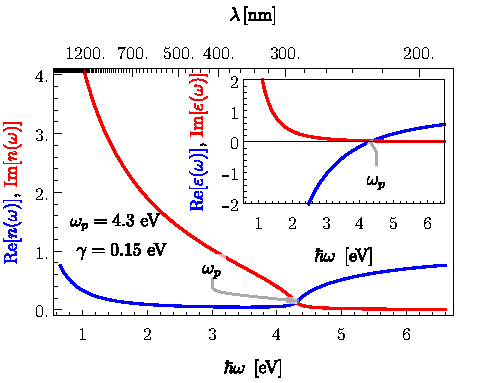
\includegraphics[scale=1. ]{0-varepsn4eV.pdf}\end{subfigure}
	\begin{subfigure}{.01\linewidth}\caption{}\label{sfig:Drude10eV}\vspace{3.75cm}\end{subfigure}\hspace*{-1em}
	\begin{subfigure}{.45\linewidth}\centering 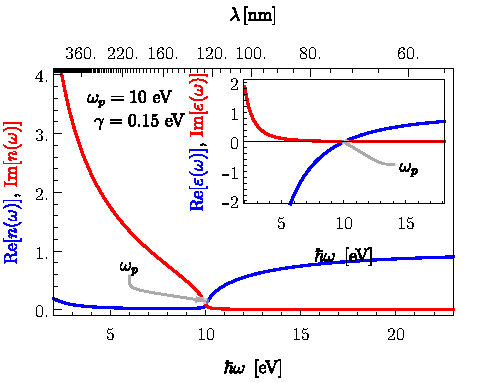
\includegraphics[scale=1. ]{0-varepsn10eV.pdf}\end{subfigure}
	\caption{ Índice de refracción (gráfica externa) y función dieléctrica (gráfica interna) del modelo de Drude-Sommerfeld para las frecuencias de plasma \textbf{a)} $\omega_p=4. 3$ eV y \textbf{b)} $\omega_p=10$ eV; ambos casos con $\gamma=0. 15$ eV, como función de la energía.  En el marco superior se observa su dependencia en longitud de onda $\lambda$. }\label{fig:Drude}
	\end{figure}	

%El modelo de Drude-Sommerfeld se ajusta a los datos experimentales de materiales realistas, como el oro y la plara,  para frecuencias bajas como el infrarojo \cite{novotny2006principles} ($0. 8$--$1,000\,\mu$m \cite{gauglitz2002handbook}).  Sin embargo, en el espectro visible ($400$--$780$ nm \cite{gauglitz2002handbook} o $1. 59$--$3. 10$ eV) el modelo de Drude-Sommerfeld debe complementarse pues la radiación EM más energética excita electrones ligados a la bada de conducción \cite{novotny2006principles}, lo que modifica la respuesta del material. 
En la Fig.  \ref{fig:nJC} se muestran los resultados experimentales para el índice de refracción de bulto del oro [Fig.  \ref{sfig:nAuJC}] y de la plata [Fig.  \ref{sfig:nAgJC}], obtenidos de  \cite{johnson1972contants}.  Los datos experimentales muestran una respuesta cualitativa semejante al modelo de Drude-Sommerfeld (Fig.  \ref{fig:Drude}) para energías bajas: energías menores a $2. 50$ eV para el oro y menores a $3. 5$ eV para la plata. % En las regiones de mayor energía, la parte imaginaria del ínidice de refracción no tiende a cero, como sí lo hace en el modelo de Drude-Sommerfeld. 

\begin{figure}[b!]\centering
	\begin{subfigure}{.01\linewidth}\caption{}\label{sfig:nAuJC}\vspace{4cm}\end{subfigure}\hspace*{-1em}
	\begin{subfigure}{.46\linewidth}\centering 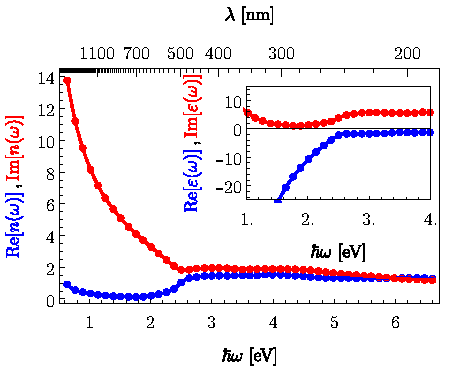
\includegraphics[scale=1.05]{0-varepsn_JC_Au.pdf}\end{subfigure}
	\begin{subfigure}{.01\linewidth}\caption{}\label{sfig:nAgJC}\vspace{4cm}\end{subfigure}\hspace*{-1em}
	\begin{subfigure}{.45\linewidth}\centering 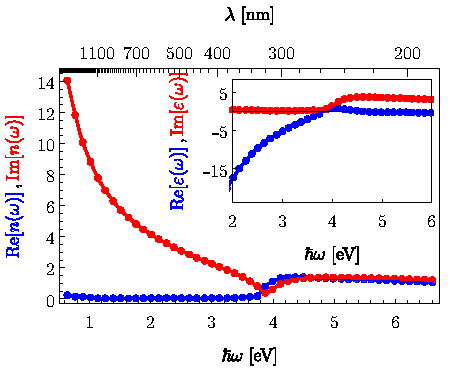
\includegraphics[scale=1.05]{0-varepsn_JC_Ag.pdf}\end{subfigure}
	\caption{ Gráficas del índice de refracción (gráfica externa) y de la función dieléctrica (gráfica interna)  \textbf{a)} del oro y \textbf{b)} de la plata,  como función de la energía.  En el marco superior se observa su dependencia en longitud de onda $\lambda$.  Los puntos en ambas gráficas corresponden a los datos experimentales obtenidos de \cite{johnson1972contants} y las líneas continuas son sólo una ayuda visual al lector. }\label{fig:nJC}
	\end{figure}	


	\subsection{Solución de Mie: esparcimiento de luz por partículas esféricas}
	
El problema de absorción y esparcimiento de luz por una partícula esférica fue resuelto por el físico alemán Gustav Mie en 1908 \cite{mie1908metallosung}.  La solución de Mie consiste en expandir una onda plana, que ilumina a una esfera de tamaño y material arbitrario, en una base de armónicos esféricos vectoriales, que son una base ortogonal esférica cuyos elementos son solución a las ecuaciones de Maxwell \cite{bohren1998absorption}.  Los campos EMs dentro de la partícula y los campos esparcidos por ésta se calculan, en la base de los armónicos esféricos vectoriales, al considerar las condiciones de contorno que satisfacen los campos EMs sobre la superficie de la esfera; los coeficientes de los campos EMs esparcidos e internos se conocen como los coeficientes de Mie \cite{bohren1998absorption}.  Existen publicaciones previas a la de Mie en donde el mismo enfoque es empleado \cite{horvath2009historic} sin embargo, en el trabajo de Mie se  desarrollan relaciones recursivas que facilitan el cálculo numérico y se discute la convergencia de este resultado \cite{horvath2009historic}.  De esta forma, en el artículo de Mie se exponen diez casos prácticos, a diferencia de otros trabajos \cite{horvath2009historic}. 

	\begin{figure}[b!]\centering
	%Angle Definitions
	%-----------------
	%set the plot display orientation
	%synatax: \tdplotsetdisplay{\theta_d}{\varphi_d}
		\tdplotsetmaincoords{60}{110}
	%
	%define polar coordinates for some vector
	%TODO: look into using 3d spherical coordinate system
		\pgfmathsetmacro{\rvec}{1. 3}
		\pgfmathsetmacro{\thetavec}{30}
		\pgfmathsetmacro{\varphivec}{60}
	\begin{subfigure}{.01\linewidth}\caption{}\label{sfig:MieParticle}\vspace{6cm}\end{subfigure}\hspace*{-1em}	
	\begin{subfigure}{.35\linewidth}	
\begin{tikzpicture}[scale=4,tdplot_main_coords]

%set up some coordinates 
	\coordinate (O) at (0,0,0);

%determine a coordinate (P) using (r,\theta,\varphi) coordinates.   This command
%also determines (Pxy), (Pxz), and (Pyz): the xy-, xz-, and yz-projections
%of the point (P). 
%syntax: \tdplotsetcoord{Coordinate name without parentheses}{r}{\theta}{\varphi}
	\tdplotsetcoord{P}{\rvec}{\thetavec}{\varphivec}

%draw figure contents
%--------------------

%Draw the NP
	\draw[tdplot_screen_coords,ball color=yellow, opacity = 1] (O) circle (. 25);
	\draw[color=blue, -, thick] (0,0,0) -- (. 18,-. 18,. 18);	
	\node at (. 09,-. 09,. 15){\color{blue} $a$};
	\node at (. 25,-. 25,-. 05){$n_m$};
	\node at (. 01,-. 18,-. 1){$n_p$};		
	
%draw the main coordinate system axes
	\draw[thick,- latex] (0,0,0) -- (. 8,0,0) node[anchor=north east]{$x$};
	\draw[thick,- latex] (0,0,0) -- (0,. 8,0) node[anchor=north west]{$y$};
	\draw[thick,- latex] (0,0,0) -- (0,0,. 8) node[anchor=south]{$z$};

%draw a vector from origin to point (P) 
	\draw[thick,color=green, - latex] (O) -- (P);
	\node at (1,. 6,1. 2) {\color{green} $\vb{r}$};
	
%draw projection on xy plane, and a connecting line
	\draw[dashed, color=green] (O) -- (Pxy);
	\draw[dashed, color=green] (P) -- (Pxy);
	\fill[green, opacity = . 3] (O) --(Pxy)-- (P)--(O);	

%draw the angle \varphi, and label it
	%syntax: \tdplotdrawarc[coordinate frame, draw options]{center point}{r}{angle}{label options}{label}
	\tdplotdrawarc[- latex]{(O)}{0. 6}{0}{\varphivec}{anchor=north}{$\varphi$}


%set the rotated coordinate system so the x'-y' plane lies within the
	%"theta plane" of the main coordinate system
	%syntax: \tdplotsetthetaplanecoords{\varphi}
	\tdplotsetthetaplanecoords{\varphivec}

%draw theta arc and label, using rotated coordinate system
	\tdplotdrawarc[tdplot_rotated_coords, - latex]{(0,0,0)}{0. 6}{0}{\thetavec}{anchor=north east}{$\theta$}

% Plane Wave
	\foreach \i in {-3,...,3}{
		\draw[thick,tdplot_screen_coords,red, - latex] (\i/10,-1,0)--(\i/10,-.5,0);}
	\node[tdplot_screen_coords] at (4/10,-.5,0){\color{red}$\vb{k}_i$};
	\node[tdplot_screen_coords] at (7/10,-.9,0){\color{red}Haz incidente};
\end{tikzpicture}
%
	\end{subfigure}
	\begin{subfigure}{.01\linewidth}\caption{}\label{sfig:MiePlane}\vspace{6cm}\end{subfigure}%\hspace*{-1em}
	\begin{subfigure}{.45\linewidth}
\begin{tikzpicture}[scale=3.5,tdplot_main_coords]
%draw the NP
	\draw[tdplot_screen_coords,ball color=yellow, opacity = 1] (O) circle (.05);


%set up some coordinates 
	\coordinate (O) at (0,0,0);

%determine a coordinate (P) using (r,\theta,\varphi) coordinates.   This command
%also determines (Pxy), (Pxz), and (Pyz): the xy-, xz-, and yz-projections
%of the point (P). 
%syntax: \tdplotsetcoord{Coordinate name without parentheses}{r}{\theta}{\varphi}
	\tdplotsetcoord{P}{\rvec}{\thetavec}{\varphivec}

%draw figure contents
%--------------------
%draw the main coordinate system axes
	\draw[thick,- latex] (0,0,0) -- (1. 5,0,0) node[anchor=north east]{$x$};
	\draw[thick,- latex] (0,0,0) -- (0,1. 5,0) node[anchor=north west]{$y$};
	\draw[thick,- latex] (0,0,0) -- (0,0,1. 5) node[anchor=south]{$z$};

%draw the main cartesian vector system 
	\draw[thick,- latex, blue] (0,0,0) -- (1,0,0) node[anchor= south east]{$\vu{e}_x$};
	\draw[thick,- latex, blue] (0,0,0) -- (0,1,0) node[anchor=north west]{$\vu{e}_y$};
	\draw[thick,- latex, blue] (0,0,0) -- (0,0,1) node[anchor= east]{$\vu{e}_z$};

%draw a vector from origin to point (P) 
	\draw[thick,color=green, - latex] (O) -- (P);
	\node at (1,. 5,1. 1) {\color{green} $\vb{r}$};

%draw projection on xy plane, and a connecting line
	\draw[dashed, color=green] (O) -- (Pxy);
	\draw[dashed, color=green] (P) -- (Pxy);
	\fill[green, opacity = . 3] (O) --(Pxy)-- (P)--(O);
	\node at (1,1. 5,1. 1) {\color{green}\bf Plano de esparcimiento};


%draw the angle \varphi, and label it
	%syntax: \tdplotdrawarc[coordinate frame, draw options]{center point}{r}{angle}{label options}{label}
	\tdplotdrawarc[- latex]{(O)}{0. 5}{0}{\varphivec}{anchor=south}{$\varphi$}


%set the rotated coordinate system so the x'-y' plane lies within the
	%"theta plane" of the main coordinate system
	%syntax: \tdplotsetthetaplanecoords{\varphi}
	\tdplotsetthetaplanecoords{\varphivec}

%draw theta arc and label, using rotated coordinate system
	\tdplotdrawarc[tdplot_rotated_coords, - latex]{(0,0,0)}{0. 45}{0}{\thetavec}{anchor=north}{$\theta$}

%draw some dashed arcs, demonstrating direct arc drawing
	\draw[dashed,tdplot_rotated_coords] (\rvec,0,0) arc (0:90:\rvec);
	\draw[dashed] (\rvec,0,0) arc (0:90:\rvec);

%set the rotated coordinate definition within display using a translation
%coordinate and Euler angles in the "z(\alpha)y(\beta)z(\gamma)" euler rotation convention
%syntax: \tdplotsetrotatedcoords{\alpha}{\beta}{\gamma}
	\tdplotsetrotatedcoords{\varphivec}{\thetavec}{0}

%translate the rotated coordinate system
%syntax: \tdplotsetrotatedcoordsorigin{point}
	\tdplotsetrotatedcoordsorigin{(P)}

%use the tdplot_rotated_coords style to work in the rotated, translated coordinate frame
	\draw[thick,tdplot_rotated_coords,- latex, purple] (0,0,0) -- (. 3,0,0) node[anchor=north west]{{\color{black}$\vu{e}_\theta,$}$\vu{e}_{\parallel,s}$};
	\draw[thick,tdplot_rotated_coords,- latex,black] (0,0,0) -- (0,. 3,0) node[anchor=west]{$\vu{e}_\varphi$};
	\draw[thick,tdplot_rotated_coords,- latex,purple] (0,0,0) -- (0,-. 3,0) node[anchor= north west]{$\vu{e}_{\perp,s}$};
	\draw[thick,tdplot_rotated_coords,- latex] (0,0,0) -- (0,0,. 3) node[anchor=south]{$\vu{e}_r$ };



%set the rotated coordinate definition within display using a translation
%coordinate and Euler angles in the "z(\alpha)y(\beta)z(\gamma)" euler rotation convention
%syntax: \tdplotsetrotatedcoords{\alpha}{\beta}{\gamma}
	\tdplotsetrotatedcoords{\varphivec}{0}{0}

%translate the rotated coordinate system
%syntax: \tdplotsetrotatedcoordsorigin{point}
	\tdplotsetrotatedcoordsorigin{(Pxy)}

	\draw[thick,tdplot_rotated_coords,- latex, purple] (0,0,0) -- (. 3,0,0) node[anchor= west]{$\vu{e}_{\parallel,i}$};
	\draw[thick,tdplot_rotated_coords,- latex, blue] (0,0,0) -- (0,0,. 3) node[anchor= west]{$\vu{e}_z$};	
	\draw[thick,tdplot_rotated_coords,- latex, purple] (0,0,0) -- (0,-. 3,0) node[anchor= north west]{$\vu{e}_{\perp,i}$};



% Plane Wave
	\foreach \i in {-7,...,-2}{
		\draw[thick,tdplot_screen_coords,red, - latex] (\i/10,0,0)--(\i/10,1,0);}
	\node[tdplot_screen_coords] at (-4.5/10,1.1,0){\color{red}$\vb{k}_i$};
	\node[tdplot_screen_coords] at (-4.5/10,-.1,0){\color{red}Haz incidente};
\end{tikzpicture}
%
\end{subfigure}
		\caption{ \textbf{a)} Diagrama de una esfera de radio $a$ e ínidce de refracción $n_p$, inmersa en una matriz con índice $n_m$ e iluminada por una onda plana con dirección de propagación $\vb{k}_i$; la dirección $\vu{e}_z$ del sistema coordenado se alinea con $\vb{k}_i$.   \textbf{b)} Diagrama del plano de esparcimiento (en verde) definido por el vector $\vb{r}$, posición donde se evalúan los campos EMs, y el vector $\vu{e}_z$.  La base canónica cartesiana para vectores se muestra en azul, mientras que la base canónica esférica se muestra en negro.  Las direcciones paralelas $\parallel$ y perpendiculares $\perp$ al plano de incidencia  para el campo eléctro incidente, denotado por el subíndice $i$ y el esparcido, denotado por el subíndice $s$ se muestran en morado.  En ambas figuras, el haz incidente se muestra en rojo. }\label{fig:Mie}
	\end{figure} 
	
Como caso particular a la solución de Mie, se considera una partícula esférica de radio $a$ no magnética, es decir, con índice de refracción es $n_p = \sqrt{\varepsilon_p}$,  inmersa en  una matriz con un índice de refracción $n_m$ e  iluminada por una onda plana $\vb{E}^i$.  Si la onda plana tiene una amplitud $E_0$, una longitud de onda $\lambda$, está  polarizada en el eje $\vu{e}_x$ y se propaga en la dirección $\vu{e}_z$ (ver Fig.  \ref{sfig:MieParticle}), su expresión en la base cartesiana canónica es $E_0 e^{i(\vb{k}_i\cdot\vb{r} - \omega t)}\vu{e}_x$, con el vector de onda $\vb{k}_i = (2\pi n_m/\lambda) \vu{e}_z$.  Al reescribir la misma onda plana en la base de los armónicos esféricos vectoriales empleada en la solución de Mie, ésta adquiere la forma \cite{bohren1998absorption}
	\begin{equation}
\vb{E}^i = E_0 \sum_{\ell=1}^\infty  i^\ell\frac{2\ell+1}{\ell(\ell+1)} \left( \vb{M}_{o1\ell}^{(1)} - i \vb{N}_{e1\ell}^{(1)}   \right),\label{eq:OndaPlana}
	\end{equation}
en donde se omite la dependencia temporal $e^{-i\omega t}$ y los términos $\vb{M}_{o1\ell}^{(1)}$ y $\vb{N}_{e1\ell}^{(1)}$ son dos elementos de los armónicos esféricos vectoriales  \cite{bohren1998absorption}, en donde el superíndice $(1)$ denota que se emplea la función $j_\ell ( k r)$ esférica de Bessel de primer tipo para la parte radial dado que la onda plana no diverge en $r = 0$.  Al proponer el campo eléctrico esparcido como
\begin{align}
\vb{E}^s &= E_0 \sum_{\ell=1}^\infty  i^\ell\frac{2\ell+1}{\ell(\ell+1)} \left(i a_\ell \vb{N}_{e1\ell}^{(3)} - b_\ell \vb{M}_{o1\ell}^{(3)}   \right), \label{eq:Es}
\end{align}
donde $\vb{M}_{o1\ell}^{(3)}$ y $\vb{N}_{e1\ell}^{(3)}$ son dos elementos de los armónicos esféricos vectoriales \cite{bohren1998absorption}, en donde el superíndice $(3)$ denota que se emplea la función $h_\ell^{(1)}(k r)$ de Hankel de primer tipo que corresponde a una onda esférica saliente en el límite asintótico, y  los coeficientes  $a_\ell$ y $b_\ell$ se calculan al considerar las condiciones de contorno del campo eléctrico sobre la interfaz entre la esfera y la matriz, dados por \cite{bohren1998absorption}
	\begin{subequations}
	\begin{align}
	a_\ell &= \frac{m\psi_\ell(mx)\psi_\ell'(x)-\psi_\ell(x)\psi_\ell' (mx)}
				{m\psi_\ell(mx)\xi_\ell'(x)-\xi_\ell(x)\psi_\ell'(mx)},
				\label{eq:an}\\
	b_\ell &= \frac{\psi_\ell(mx)\psi_\ell'(x)-m\psi_\ell(x)\psi_\ell' (mx)}
			{\psi_\ell(mx)\xi_\ell'(x)-m\xi_\ell(x)\psi_\ell'(mx)},
			 \label{eq:bn}
	\end{align}			 
	\label{eq:MieCoef}
	\end{subequations}
\hspace*{-.5em}en donde $m = n_p/n_m$ es el cociente entre los índices de refracción, $x = k_m a$ es el parámetro de tamaño con $k_m = n_m(2\pi/\lambda)$, y $\psi_\ell$ y $\xi_\ell$  son las funciones de Riccati-Bessel \cite{bohren1998absorption}; los términos $\psi'_\ell$ y $\xi'_\ell$ denotan las derivadas de las funciones respecto a su argumento.  Las funciones de Ricatti-Bessel, en términos de  $j_\ell(\rho)$, la función de Bessel esférica de primer tipo y $h_\ell^{(1)}(\rho)$, la función de Hankel de primer tipo,  está dadas como \cite{bohren1998absorption,arfken2001methods}
	\begin{align*}
	\psi_\ell (\rho) = \rho j_\ell (\rho)
	\hspace{2cm}\mbox{y}\hspace{2cm}
	\xi_\ell (\rho) = \rho h_\ell ^{(1)}(\rho). 
	\end{align*}
Los armónicos esféricos vectoriales representan una expansión multipolar del campo eléctrico esparcido por una partícula esférica y los coeficientes de Mie [Ec.  \eqref{eq:MieCoef}] modulan la contribución al campo total esparcido de cada término:  $a_\ell$, los multipolos eléctricos; $b_\ell$, los magnéticos \cite{kreibig1995clusters}. 

Al descomponer el campo eléctrico es una componente paralela, denotada por $\parallel$, y en una transversal, denotada por $\perp$, al plano generado por el eje $\vu{e}_z$ y el punto a evaluar $\vb{r}$, denominado plano de incidencia [ver Fig.  \ref{sfig:MiePlane}], el campo eléctrico incidente $\vb{E}^i$ [Ec.  \eqref{eq:OndaPlana}] se relaciona con el campo eléctrico  esparcido por una esfera $\vb{E}^s$ [Ec.  \eqref{eq:Es}]   mediante la matriz de esparcimiento $\mathbb{S}$, es decir, se cumple que
	\begin{equation}
	\mqty(E_{\parallel}^s\\ E_{\perp}^s) = \frac{e^{ik(r-z)}}{-ikr} \mqty(\dmat[0]{S_2,S_1})\mqty(E_{\parallel}^i\\ E_{\perp}^i),
	\label{eq:ScatterMat}
	\end{equation}
donde los elementos de la matriz de esparcimiento $S_1$ y $S_2$ son \cite{bohren1998absorption}
	\begin{subequations}	
	\begin{align}
	S_1(\theta) = \sum_\ell \frac{2\ell+1}{\ell(\ell+1)} [a_\ell\pi_\ell (\cos\theta)+ b_\ell\tau_\ell(\cos\theta)], \label{eq:S1}\\
	S_2 (\theta)= \sum_\ell \frac{2\ell+1}{\ell(\ell+1)} [a_\ell\tau_\ell(\cos\theta) + b_\ell\pi_\ell(\cos\theta)], \label{eq:S2}
	\end{align}\label{eq:SMatElements}
	\end{subequations}
\hspace{-.5em}donde $\theta$ es el ángulo donde se evalúan los campos EMs medido desde la dirección de propagación de la onda plana [ver Fig.  \ref{sfig:MiePlane}], y la dependencia angular está dada por las funciones
	\begin{align*}
	\pi_\ell(\cos\theta)= \frac{P_\ell^1(\cos\theta)}{\sin\theta},
	\hspace{2cm}\mbox{y}\hspace{2cm}
	\tau_\ell(\cos\theta) = \dv{P_\ell^1(\cos\theta)}{\theta},
	\end{align*}
con $P_\ell^m$   las \emph{funciones asociadas de Legendre}\footnote{Se toma la convención de que estas funciones no están normalizadas, es decir, se cumple que la relación de ortogonalidad es $\int_{-1}^1 P_\ell^m(\mu)P_{\ell'}^m(\mu)d\mu = \delta_{\ell,\ell'} \frac{2}{\ell+1}\frac{(\ell+m)!}{(\ell-m)!},$ con $\mu=\cos\theta$}  de grado $\ell$ y orden $m$ \cite{bohren1998absorption,arfken2001methods}.  Las relaciones de recurrencia de las funciones asociadas de Legendre \cite{arfken2001methods} permiten expresar a  $\pi_\ell$ y $\tau_\ell$ como  
	\begin{align*}
	\pi_\ell(\mu) = \frac{2\ell-1}{\ell-1} \mu \pi_{\ell-1}(\mu) - \frac{\ell}{\ell-1}\pi_{\ell-2}(\mu)
	\hspace{1cm}\mbox{y}\hspace{1cm}
	\tau_\ell(\mu) = \ell \mu\pi_\ell(\mu) - (\ell+1)\pi_{\ell-1}(\mu),
	\end{align*}
%	\eqhalf{\pi_\ell(\cos\theta) = \frac{(2\ell-1) \cos\theta \pi_{\ell-1}(\cos\theta) - \ell \pi_{\ell-2}(\cos\theta)}{\ell-1},\notag }
%	\eqhalf{\tau_\ell(\cos\theta) = \ell \cos\theta\pi_\ell(\cos\theta) - (\ell+1)\pi_{\ell-1}(\cos\theta),\notag}
%
%\noindent
en donde se empleó el cambio de variable $\mu = \cos\theta$ y se define   $\pi_0 =0 $ y $\pi_1 = 1$. 
	
	El campo esparcido [Ec.  \eqref{eq:Es}] está en términos de los coeficientes $a_\ell$ y $b_\ell$ [Ecs.  \eqref{eq:MieCoef}], que dependen, entre otros parámetros, del índice de refracción de la partícula.  De la Ec.  \eqref{eq:Es} se observa que, para un multipolo $\ell$ fijo, la contribución del campo eléctrico es máxima cuando el denominador de los coeficientes de Mie es mínimo \cite{novotny2006principles}.  Si se considera que la respuesta óptica de la partícula es 	$\varepsilon_p (\omega) = n_p^2 (\omega)$, y se fijan los parámetros $a$, $n_m$ y $\lambda$, 	entonces a la frecuencia $\omega_\ell = c (2\pi / \lambda_\ell)$, donde el denominador de las Ecs.  \eqref{eq:MieCoef} es nulo, se le denomina \emph{modo normal} de orden $\ell$ \cite{bohren1998absorption,maciel2017momentum}.  Los modos normales eléctricos ocurren a las frecuencias en las que se cumple la condición 
	\begin{align}
	\psi_\ell(mx)\xi_\ell'(x)-m\xi_\ell(x)\psi_\ell'(mx) = 0. 
	\label{eq:an_resonance}
	\end{align}
Al considerar el límite de partícula pequeña ($x\ll 1$) para esferas inmersas en vacío ($n_m=1$), haciendo un desarrollo en serie de Taylor de las funciones de Bessel y Hankel al rededor del origen y sustituyéndolas en la Ec.  \eqref{eq:an_resonance}, se obtiene que los modos normales eléctricos cumplen la relación \cite{maciel2017momentum}
	\begin{equation}
	\varepsilon_p(\omega_\ell) = - \frac{\ell+1}{\ell}.  
	\label{eq:NormalModes}
	\end{equation}

	\begin{figure}[b!]\centering
		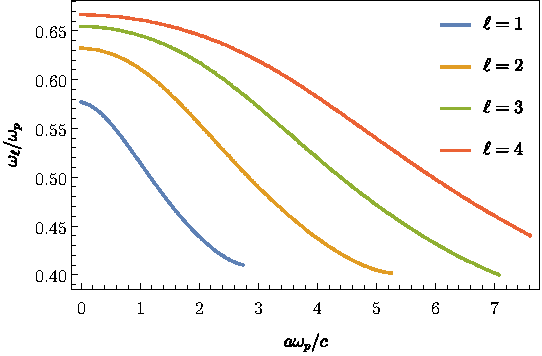
\includegraphics[scale=1]{0-DrudeMultipoles.pdf}
	\caption{Frecuencias de resonancia $\omega_\ell/\omega_p$ para una esfera con una función dieléctrica tipo Drude, como función del parámetro adimensional  $\omega_p a / c$, para los multipolos $\ell = 1,2,3$ y $4$. }
	\label{fig:NormalModes}
	\end{figure}			
	
Si se emplea la función dieléctrica del modelo de Drude-Sommerfeld [Ec.  \eqref{eq:Drude}] para $\omega = \omega_\ell$	y se sustituye en la Ec.  \eqref{eq:NormalModes}, al despejar $\omega_\ell$ tras considerar además el límite $\gamma\to 0$, la expresión para la frecuencia de resonancia del  modo normal del multipolo $\ell$ es \cite{maciel2017momentum}
	\begin{equation}
	\frac{\omega_\ell}{\omega_p} = \sqrt{ \frac{\ell}{2\ell+1}}.  \label{eq:PPequeña}
	\end{equation}
	
Para partículas esféricas de radio arbitrario $a$ con una función dieléctrica dada por el modelo de Drude-Sommerfeld, la frecuencia de resonancia $\omega_\ell$ sufre un corrimiento al rojo debido al tiempo de acomplamiento $a/c$ entre la interacción EM de la esfera y  la densidad de carga inducida que corresponde al plasmón de superficie \cite{aizpurua1998coupling}.  En la Fig.  \ref{fig:NormalModes} se muestran las frecuencias de resonancia $\omega_\ell$ normalizadas respecto a la frecuancia de plasma $\omega_p$, como función del parámetro adimensional $a\omega_p / c$ para los multipolos $\ell = 1,2,3$ y $4$.  El límite de partícula pequeña [Ec.  \eqref{eq:PPequeña}]	se recupera cuando  $a\to 0$ (lado izquierdo de la gráfica en la Fig.  \ref{fig:NormalModes}).  Para una función dieléctrica arbitraria, los modos normales se calculan como la frecuencia a la que la partícula extingue\footnote{Extinción se entiende como la pérdida de luz ocacionada por la absorción y esparcimiento de luz de la partícula; esta relación es conocida como el  \emph{teorema óptico} \cite{bohren1998absorption}. } la mayor cantidad de luz \cite{kreibig1995clusters}. 	
	
	\subsection{Modelo de esparcimiento coherente}

	La nanoplasmónica estudia la respuesta EM a escala nanométrica \cite{novotny2006principles} y, por sus crecientes aplicaciones, se busca entender y manipular los mecanismos físicos a esta escala \cite{sihvola2007dielectric}.  En el modelado de la respuesta EM de materiales nanométricos heterogéneos ---como una monocapa de NPs esféricas--- existen enfoques como la aproximación cuasi-estática \cite{sihvola1999mixing}, la cual es válida para partículas pequeñas ($x\ll 1$), que permite la homogenización del material mediante una teoría de medio efectivo donde las partículas son tratadas como dipolos puntuales \cite{sihvola1999mixing,pena-gomar2006coherent}.  Para partículas grandes, la respuesta EM espacial no se desacopla de la respuesta temporal por lo que se consideran, además del dipolo, ordenes multipolares mayores  \cite{sihvola1999mixing}, es decir, se emplea una teoría de esparcimiento 	 \cite{pena-gomar2006coherent}. 
	
	El modelo de esparcimiento coherente (CSM) es una teoría de  esparcimiento que calcula el campo eléctrico total esparcido por una monocapa de NPs  esféricas desordenadas de radio arbitrario, suspendida en un medio no absorbente, ante la incidencia de una onda plana \cite{reyes2018analytical}. 	El CSM proporciona expresiones de reflectancia y transmitancia al considerar el campo eléctrico esparcido tiene dos componentes: una coherente ---respuesta promedio con una dirección de propagación bien definida--- y una  difusa ---causada por las fluctuaciones y cuya propagación es en todas las direcciones--- \cite{reyes2018analytical}; la dirección del haz coherente reflejado obedece la ley de reflexión $\theta_i = \theta_r$, mientras que el transmitido obedece la la ley de Snell $n_i\sin\theta_i = n_t\sin\theta_t$ \cite{garcia2012multiple}, en donde $\theta_i$ es el ángulo de incidencia; $\theta_r$, el de reflexión y $\theta_t$, el de transmisión.  En el CSM se considera que la energía que transporta el haz difuso es mucho menor en comparación a la energía trasnportada por el haz coherente \cite{reyes2018analytical}.  
	
%	 El CSM considera la componente coherente del esparcimiento de cada una de los NPs presentes en una monocapa, según la solución de Mie, y dota de propiedades ópticas a una superficie matemática de grosor nulo que sustituyen a la monocapa de NPs.  Las NPs son tratadas como esparcidores puntuales ante la presencia de un campo eléctrico promedio \cite{reyes2018analytical}, que incluye la contribución del esparcimiento multiple debido a la interacción entre las NPs \cite{garcia2012multiple}.  Para calcular la respuesta óptica de la superficie matemática, se considera primero una monocapa suspendida (FSM), inmersa en un dieléctrico como se muestra en la Fig.  \ref{fig:FSM}, y luego se incluye la contribución del sustrato [ver Fig.   \ref{fig:ATR}] mediante procesos de multiples reflexiones \cite{reyes2018analytical}.  
    
	\begin{figure}[h!]\centering
	\begin{subfigure}{.05\textwidth}\vspace{-4.5cm}\caption{}\label{fig:FSM}\end{subfigure}
	\begin{subfigure}{.43\textwidth}
\begin{tikzpicture}[scale=.75]
\def\a{. 5}
\def\d{. 5}

\foreach \x in {-4,-2. 9,-1. 1,0,1. 2,2. 4,3. 8}{
\fill[ball color=yellow, opacity=1] (\x,0) circle(\a);}


\draw[thick, dashed] (-4. 5,-\d) rectangle (4. 5,\d);

\draw[latex -, thick, red, line width=2. 5](135:1)--(135:4) node[anchor=south west]{$\vb{k}_i$};
\draw[- latex, thick, red, line width=2. 5](45:1)--(45:4)node[anchor=north west]{$\vb{k}_{r,coh}$};

\draw[- latex, thick, blue] (0,0)--(90:2) node[anchor = south]{$z$};
\draw[- latex, thick, blue] (0,0)--(0:2) node[anchor = west]{$x$};
\path (0,0)++(135/2:1. 5)node[anchor=south west, blue]{$\theta$}; 
\draw[- latex, thick, blue](90:1. 5)arc(90:45:1. 5);
\path (0,0)++(90+45/2:1. 5)node[anchor=south east, blue]{$\theta$}; 
\draw[- latex, thick, blue](90:1. 5)arc(90:135:1. 5);

\draw[- latex, thick, purple] (0,0)--(-45:1. 5) node[anchor = west]{$z'$};
\draw[- latex, thick, purple] (0,0)--(-135:1. 5) node[anchor = east]{$x'$};
\path (0,0)++(30:1. 2)node[anchor=south west, purple]{$\theta'$}; 
\path (0,0)++(30:1. 2)node[anchor=south west, blue]{$\;\;\; =  \pi - 2\theta$}; 
\draw[- latex, thick, purple](-45:1. 2)arc(-45:45:1. 2);

\node at (-4,1) {$\; n_m$};
\node at (-4,0) {$\; n_p$};
\end{tikzpicture}
	\end{subfigure}
	\begin{subfigure}{.05\textwidth}\vspace{-4.5cm}\caption{}\label{fig:ATR}	\end{subfigure}
	\begin{subfigure}{.43\textwidth} 
\begin{tikzpicture}[scale=.75]
\def\a{. 5}
\def\d{. 5}

\fill[blue, opacity=. 25] (-4. 5,-4\d) rectangle (4. 5,-\d);

\foreach \x in {-4,-2. 9,-1. 1,0,1. 2,2. 4,3. 8}{
\fill[ball color=yellow, opacity=1] (\x,0) circle(\a);}


\draw[thick, dashed] (-4. 5,-\d) rectangle (4. 5,\d);

\draw[latex -, thick, red, line width=2. 5](0,0)--(-120:. 5)--(-140:4) node[anchor=north west]{$\vb{k}_i$};
\draw[- latex, thick, red, line width=2. 5](0,0)--(-60:. 5)--(-40:4)node[anchor=north east]{$\vb{k}_{r,coh}$};

\draw[- latex, thick, blue] (0,0)--(-90:3. 5) node[anchor = north]{$-z$};
\draw[- latex, thick, blue] (0,0)--(0:2. 75) node[anchor = west]{$x$};

\path (0,0)++(-90:2. 5)node[anchor=north east, blue]{$\theta_i$}; 
\draw[- latex, thick, blue](-90:2. 5)arc(-90:-45:2. 5);
\path (0,0)++(-90:2. 5)node[anchor=north west, blue]{$\theta_i$}; 
\draw[- latex, thick, blue](-90:2. 5)arc(-90:-135:2. 5);

\draw[thick, blue, dashed](0,0) -- (-120:2. 25);
\draw[thick, blue, dashed](0,0) -- (-60:2. 25);
\path (0,0)++(-90-50/2:1. 6)node[anchor=north west, blue]{$\theta_t$}; 
\draw[- latex, thick, blue](-90:1. 5)arc(-90:-60:1. 5);
\path (0,0)++(-90+50/2:1. 6)node[anchor=north east, blue]{$\theta_t$}; 
\draw[- latex, thick, blue](-90:1. 5)arc(-90:-120:1. 5);

\draw[- latex, thick, purple] (0,0)--(60:2) node[anchor = south west ]{$z'$};
\draw[- latex, thick, purple] (0,0)--(150:2) node[anchor =  east]{$-x'$};
\path (0,0)++(30:1. 2)node[anchor=south west, purple]{$\theta'$}; 
\path (0,0)++(30:1. 2)node[anchor=south west, blue]{$\;\;\; =  \pi - 2\theta_t$}; 
\draw[- latex, thick, purple](60:1. 2)arc(60:-60:1. 2);

\node at (-3. 75,2) {(Aire)};
\node at (-4,1) {$\; n_m$};
\node at (-4,0) {$\; n_p$};
\node at (-4,-1) {$\; n_s$};
\node at (-3. 6,-2) {(Vidrio)};	
\end{tikzpicture}
	\end{subfigure}
	\caption{Esquema de la reflexión coeherente de una monocapa de NPs esféricas \textbf{a)} suspendida en un a matriz con índice de refracción $n_m$, y \textbf{b)} sobre un sustrato con índice de refracción $n_s$, en configuración ATR.  EL sistema coordenado azul es colocado sobre la monocapa y con el eje $z$ normal a ésta; el sistema coordenado morado se alínea,  en su dirección $z$, con la dirección de propagación de la luz al incidir sobre la NP, por lo que es el sistema coordenado empleado en la solución de Mie. }	\label{figs:CSM-Diagrams}	
	\end{figure}	
	
Las expresiones para los coeficientes de amplitud de reflexión y de transmisión para una FSM, inmersa en una matriz con índice de refracción $n_m$, donde incide una onda plana con un ángulo $\theta$ medido desde la dirección normal a la monocapa [ver Fig.  \ref{fig:FSM}], son \cite{reyes2018analytical}
	\begin{align}
	r_{coh}(\theta) &= \frac{-\alpha S_n(\pi-2\theta)}{1+\alpha S(0)+\frac14 \alpha^2 \left[S^2(0)-S_n^2 (\pi-2\theta) \right]},\label{eq:rFSM}\\
	t_{coh}(\theta) &= \frac{1-\frac14\alpha^2 \qty[S^2(0)-S^2_n(\pi-2\theta)]}{1+\alpha S(0)+\frac14 \alpha^2 \left[S^2(0)-S_n^2 (\pi-2\theta) \right]},\label{eq:tFSM}
	\end{align}
donde  $\alpha= 2\Theta/x^2\cos\theta$, con $x=k_0an_m$ el parámetro de tamaño y $\Theta$ la fracción superficial de cubierta, y donde $S_n(\theta)$ ---$n=1$ para polarización \emph{s} y $n=2$ para \emph{p}--- son los elementos de la matriz de esparcimiento, dados por las Ecs.  \eqref{eq:SMatElements}.  Los elementos de la matriz de esparcimiento se evalúan en $(\pi-2\theta)$ pues ésta es la dirección del haz reflejado respecto a la dirección del esparcimiento frontal de las NPs $S(0)$, en donde $S(0) = S_1(0)=S_2(0)$. 

%
%de incidencia del haz medido desde el sistema coordenado empleado en la solución de Mie [en morado en la Fig.  \ref{fig:FSM}]; el término $S(0)$ es independiente de la polarización, pues se cumple que $S(0) = S_1(0)=S_2(0)$ según las Ecs.  \eqref{eq:SMatElements}. 

Los coeficientes de amplitud del sistema sustrato-matriz-monocapa se calculan al considerar  múltiples reflexiones en la interfaz entre las superficies dadas por la interfaz sutrato-matriz y matriz-monocapa [ver Fig.  \ref{fig:ATR}]. Al realizar este procedimento con la presencia de un sustrato con un índice de refracción $n_s$ y al considerar una medición en una configuración ATR [ver Fig.  \ref{fig:ATR}], se obtienen las expresiones
	\begin{align}
	r &= \frac{r_{sm}(\theta_i)+r_{coh}(\theta_t)e^{i\beta}}
		{1+r_{sm}(\theta_i)r_{coh}(\theta_t)e^{i\beta}},
		\label{eq:r3CSM}\\
	t &= \frac{t_{sm}(\theta_i)+t_{coh}(\theta_t)e^{i\beta/2}}
		{1+r_{sm}(\theta_i)r_{coh}(\theta_t)e^{i\beta/2}},
		\label{eq:t3CSM}
	\end{align}
donde $\theta_i$ es el ángulo de incidencia a la interfaz, $\theta_t$ el ángulo de transmisión dado por la ley de Snell, $\beta=2 k_0 a n_m\cos\theta_t$ el cambio de fase de la luz al cruzar la monocapa, y $r_{sm}$ y $t_{sm}$ los coeficientes de amplitud de reflexión y transmisión de Fresnel para una interfaz sustrato-matriz. 

La reflectancia $R$ y transmitancia $T$ son las cantidades experimentales medidas al estudiar la respuesta óptica de la monocapa.  La reflectancia (transmitancia) es la potencia reflejada (transmitida) normalizada por la potencia incidente \cite{griffiths2013electrodynamics} y dado que la potencia es proporcional al cuadrado de la magnitud del campo eléctrico \cite{griffiths2013electrodynamics}, la reflectancia y transmitancia se relacionan con los coeficientes de amplitud [Ecs.  \eqref{eq:r3CSM} y \eqref{eq:t3CSM}] mediante la expresión 
	\begin{align}
	R &= r r^*,\label{eq:R}\\
	T &= \frac{n_m \cos\theta_t}{n_s \cos\theta_i} t t^*  ,\label{eq:T}
	\end{align}
donde  $*$ denota el complejo conjugado y el cociente en la Ec.  \eqref{eq:T} es el término de impedancia (para materiales no magnéticos) originado por el cambio de medio material en la interfaz \cite{griffiths2013electrodynamics}. 

\section{Resultados numéricos}

	Para estudiar la respuesta óptica de una monocapa de NPs plasmónicas se empleó el formalismo del CSM considerando una función dieléctrica tipo Drude [Ec. \eqref{eq:Drude}] para las NPs. El modelo de Drude-Sommerfeld se emplea en el cálculo de la reflectancia de la monocapa dado que es un modelo sencillo que considera únicamente las transiciones intrabanda de los materiales, a diferencia de los datos experimentales para el oro y la plata en donde transiciones electrónicas más complejas están presentes. Asimimo, la elección de la frecuencia de plasma $\omega_p$ y la constante fenomenológica $\gamma$ permite modificar la posición de los picos de resonancia, así como su ancho, por lo que es posible distinguir los modos normales de NPs individuales y así diferenciarlos de algún otro fenómeno, como lo puede ser uno semejante a la resonancia de red del plasmón de superficie (SPLRs) reportada en en \cite{kabashin2009plasmonic} y \cite{danilov2018ultra}.
	
	 Dado que las mediciones de la función dieléctrica del oro dependen del proceso de producción de la muestra,  existe un rango de valores para los parámetros  $\omega_p$ y $\gamma$ que ajustan una función dieléctrica tipo Drude a los datos experimentales \cite{svetovoy2008optical}. Por tanto, para los cálculos de la reflectancia de NPs plasmónicas se emplearon las funciones dieléctricas tipo de Drude con $\omega_p = 4.3$ eV y  $\gamma = 0.15$ eV para el oro [ver Fig. \ref{sfig:Drude4eV}], y $\omega_p = 10$ eV y  $\gamma = 0.15$ eV [ver Fig. \ref{sfig:Drude10eV}] para la plata.	Con el modelo de Drude simulando oro, se analiza en la primera sección el comportamiento de una monocapa de NPs suspendida (FSM)  en vacío, mientras que en la segunda sección hace el análisis de los resultados obtenidos al considerar una configuración de reflexión total atenuada (ATR) como la que se muestra en la Fig. \ref{fig:ATR1}, empleando el ajuste con el modelo de Drude-Sommerfeld para el oro y la plata.

	\subsection{Reflectancia de una monocapa suspendida en aire}
	
%\begin{itemize}
%\item hacer un corte  de un ángulo y graficar todas las fracciones de cubierta
%\end{itemize}	
	
Para el cálculo de la reflectancia de una FSM, en una matriz de aire ($n_m=1$), se empleó la Ec.  \eqref{eq:R} con el coeficiente de amplitud de reflexión coherente $r_{coh}$ [Ec.  \eqref{eq:rFSM}].  En la Fig.  \ref{fig:R-FSM} se muestran los resultados de la reflectancia $R$ como función de la longitud de onda $\lambda$ y el ángulo de incidencia $\theta_i$.  La frecuencia de plasma empleada para la función dieléctrica tipo Drude con $\omega_p = 4. 3$ eV y $\gamma = 0. 15$ eV (que corresponden a $288. 5$ nm  y $8,270$ nm respectivamente). Se consideraron NPs de radio $a=30$ nm y fracciones de cubierta $\Theta$: $0. 05$, $0. 1$, $0. 2$, $0. 3$ y $0. 4$. En la Fig.  \ref{fig:R-FSM} se muestran los resultados de $R$ para polarización \emph{p}  en las gráficas $\mathbf{i)-v)}$, mientras que los resultados de $R$ para polarización \emph{s} se muestran en las gráficas $\mathbf{vi)-x)}$. La línea vertical verde punteada en $\lambda \approx 502$ nm corresponde a la excitación dipolar ($\ell = 1$) para una partícula esférica individual y la línea vertical rosa punteada en $\lambda \approx 456$ nm lo hace al modo cuadrupolar ($\ell=2$); ambas resonancias fueron calculadas según la Fig.  \ref{fig:NormalModes}. 
					
	\begin{figure}[h!]\centering
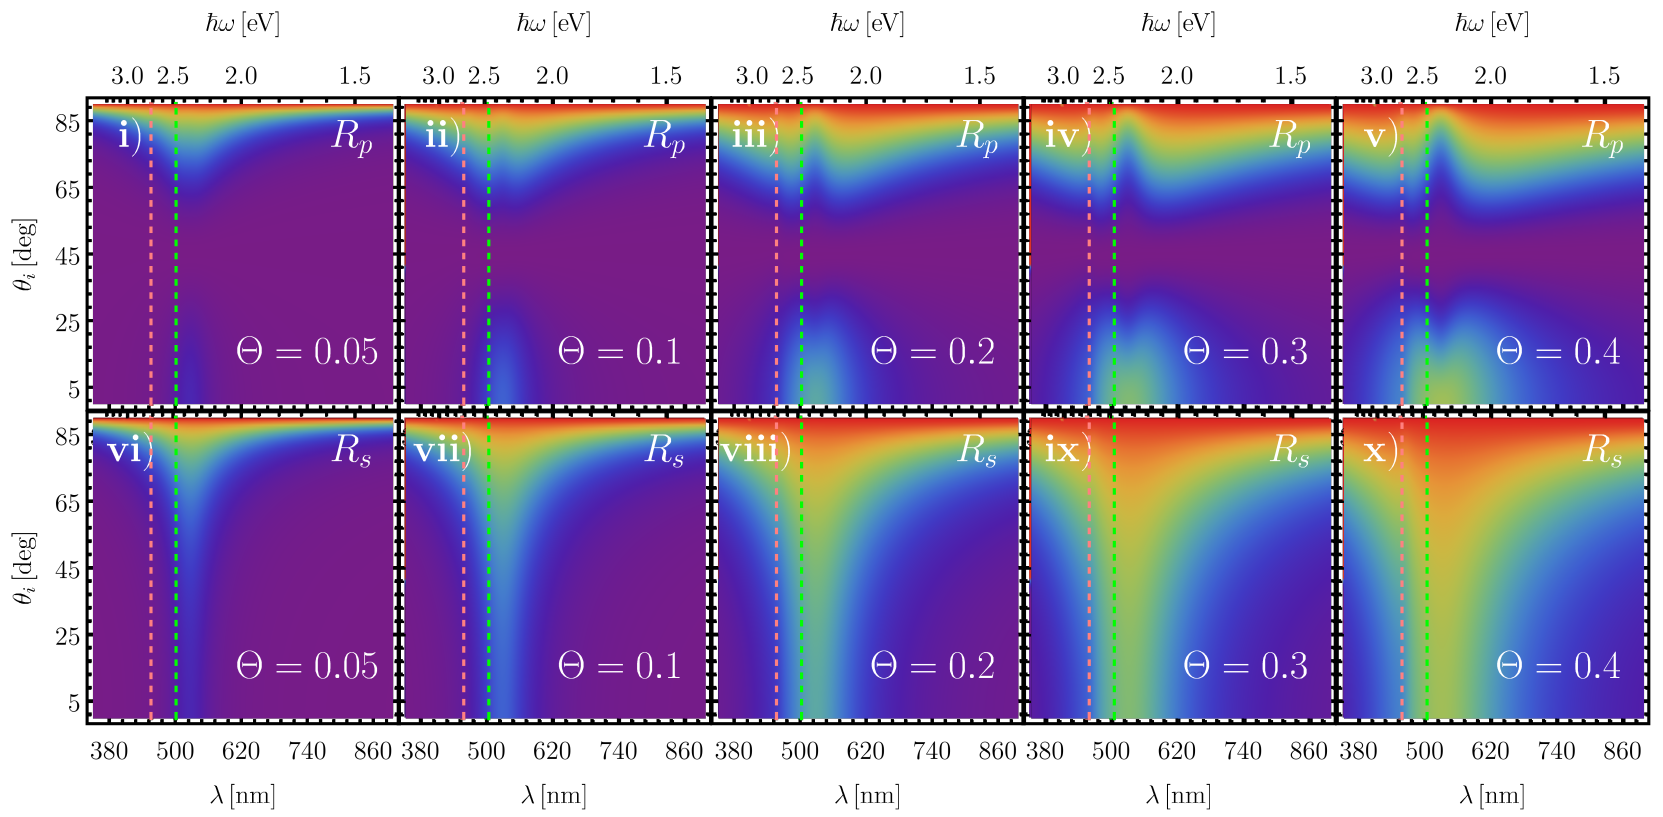
\includegraphics[width = .9\linewidth	]{4-Wp4FSMThetaVar/0-2D_Grid.png}%
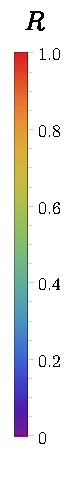
\includegraphics[scale=.85, trim={00 -5 00 00}, clip]{0-RBar_v}
	\caption{Gráficas de reflectancia para una FSM como función del ángulo de incidencia $\theta_i$ y de la longitud de onda $\lambda$ para una función dieléctrica tipo Drude con $\omega_p=4. 3$ eV  y  $\gamma=0. 15$ eV.  Las gráficas \{pol.  \emph{p} [$\mathbf{i)-v)}$] y pol.  \emph{s} [$\mathbf{i)-v)}$]\} muestran los resultados para NPs de un radio de $a=30$ nm y distintas fracciones de cubierta $\Theta$: $0. 05$, $0. 1$, $0. 2$, $0. 3$ y $0. 4$.  En el marco superior se muestra su dependencia en la energía $\hbar\omega$. }	\label{fig:R-FSM}	
	\end{figure}						
					
La reflectancia para luz polarizada en \emph{p} [Figs. \ref{fig:R-FSM} $\mathbf{i)-v)}$] es nula para el ángulo de Brewster $\theta_B \approx 41^\circ$ y para regiones alejadas de las SPRs de  partículas esféricas individuales (líneas verticales verde y rosa punteadas localizadas en $502$ nm y $456$ nm respectivamente). Para $\Theta = 0.05$ a $520$ nm se presenta un máximo en la reflectancia de $R_p$ [gráfica $\mathbf{i)}$] pero, al crecer la fracción de cubierta, a $520$ nm se presentan mínimos, como se observa en las gráficas $\mathbf{ii)-v)}$. De forma distinta, para polarización \emph{s} [Figs. \ref{fig:R-FSM} $\mathbf{vi)-x)}$] la reflectancia es apreciable para todo ángulo de incidencia a las freciencoas de las SPRs . En ambos casos, se observa que mientras la fracción de cubierta aumenta, la frontera de las regiones donde la reflectancia es apreciable crece, así como la intensidad de la luz reflejada, como se puede observar contrastando las gráficas $\mathbf{i)}$ con $\mathbf{v}$ y $\mathbf{vi)}$ con $\mathbf{x)}$. 

En la Fig. \ref{fig:FSM-Cuts} se muestran los resultados de la reflectancia graficados en la Fig. \ref{fig:R-FSM} para un ángulo de incidencia de $\theta_i = 65^\circ$, tanto para una onda incidente con polarización \emph{p} [Fig \ref{sfig:FSM-cutp}] y con polarización \emph{s} [Fig \ref{sfig:FSM-cuts}]. Para la polarización \emph{p} se presenta un mínimo en la reflectancia al rededor de $520$ nm para fracciones de cubierta mayores a $\Theta = 0.05$, mientras que para polarización \emph{s} hay un máximo en la relfectancia a $520$ nm para todas las fracciones de cubierta. Para las fracciones de cubierta mayores, $\Theta = 0.3$ y $\Theta = 0.4$,  se observa un  mínimo en la reflectancia al rededor de $460$ nm para ambas polarizaciones. Dado que las SPRs de esferas individuales estás localizadas en $502$ nm (dipolo) y $456$ nm (cuadrupolo), la respuesta de la monocapa en $540$ corresponde a un corrimiento al rojo del modo dipolar debido a la interacción de las NPs de la monocapa entre sí; lo mismo ocurre para el modo cuadrupolar.

	\begin{figure}[t!]\centering
	\begin{subfigure}{.01\linewidth}\caption{}\label{sfig:FSM-cutp}\vspace{3.75cm}\end{subfigure}\hspace*{-1em}
	\begin{subfigure}{.45\linewidth}\centering 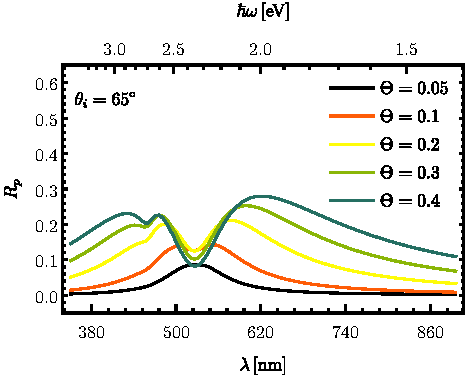
\includegraphics[scale=1. ]{4-Wp4FSMThetaVar/cut_angle_65_p.pdf}\end{subfigure}
	\begin{subfigure}{.01\linewidth}\caption{}\label{sfig:FSM-cuts}\vspace{3.75cm}\end{subfigure}\hspace*{-1em}
	\begin{subfigure}{.45\linewidth}\centering 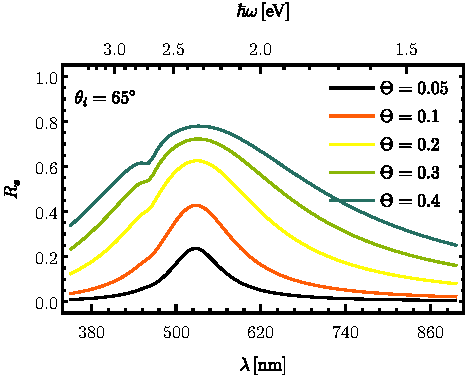
\includegraphics[scale=1. ]{4-Wp4FSMThetaVar/cut_angle_65_s.pdf}\end{subfigure}
	\caption{Gráficas de reflectancia de una FSM de NPs esféricas de radio $a$ en polarización \textbf{a)} \emph{p} y \textbf{b)} \emph{s} como función de la longitud de onda $\lambda$, para un ángulo de incidencia $\theta_i =65^\circ$. Los parámetros de la función dieléctrica tipo Drude para las NPS son $\omega_p = 4.3$ eV y $\gamma = 0.15$ eV y las fracciones de cubierta consideradas fueron $\Theta$: $0. 05$, $0. 1$, $0. 2$, $0. 3$ y $0. 4$.  En el marco superior se muestra su dependencia en la energía $\hbar\omega$.}\label{fig:FSM-Cuts}
	\end{figure}	

En las Figs. \ref{fig:R-FSM} y \ref{fig:FSM-Cuts} se observa la respuesta óptica de una monocapa de NPs suspendida en vacío al interactuar con una onda plana. Si se considera la presencia de un segundo medio además de la matriz, y que la monocapa se encuentra sobre la interfaz entre los dos medios, según los valores de los índice de refracción se hay dos casos: incidencia externa e incidencia interna. Para incidencia externa, el haz que ilumina a las NPs es una onda plana, a todo ángulo de incidencia, que se propaga dentro de la matriz, por lo que los resultados cualitativos de la reflectancia son semejantes a los de la FSM; cuantitativamente se presenta un fenómeno de apantallamiento lo cual reduce el contraste de las mediciones respecto a la FSM. Por otro lado, para el caso de incidencia interna, a ángulo mayores al ángulo crítico, se presenta el fenómeno de reflexión total interna, en donde una onda evanescente penetra el medio donde se encuntran las NPs. Cuando la onda evanescente, que decae de forma exponencial y se propaga a lo largo de la interfaz, interactúa con las NPs, se está en una configuración de reflexión total atenuada (ATR). En este caso, es la onda evanescente la que ilumina a las NPs de la monocapa y ya no una onda plana por lo que fenómenos como la apariciones de LSPs pueden modificar la respuesta óptica observada para la FSM.

				
				
	\subsection{Reflectancia de una monocapa en configuración ATR}
%
%\begin{itemize}
%\item decir que la epsilon es la de Drude
%\item cambiar la redacción para que no sea monótono
%\end{itemize}

Al emplear la Ec.  \eqref{eq:R} con el coeficiente de amplitud de reflexión $r$ de la Ec.  \eqref{eq:r3CSM} que considera la presencia de un sustrato, con índice de refracción $n_s$,  se calcula la reflectancia de una monocapa de NPs inmersa en una matriz con índice de refracción $n_m$ y que está colocada sobre el sustrato. Para comparar los resultados d la reflectancia $R$ para una FSM y una monocapa en configuración ATR, se vuelven a emplear los parámetros para la función dieléctrica tipo Drude $\omega_p = 4.3$ eV y $\gamma = 0.15$ eV, así como los índices de refracción de la matriz $n_m = 1$ y del sustrato $n_s = 1.5$. En la Fig.  \ref{fig:R-ATR4} se muestran los resultados de la reflectancia $R$ como función de la longitud de onda $\lambda$ y el ángulo de incidencia $\theta_i$, para una monocapa de NPs de radio $a=30$ nm para distintos valores de la fracción de cubierta $\Theta$: $0. 05$, $0. 1$, $0. 2$, $0. 3$ y $0. 4$, en polarización \emph{p} [en la Fig.  \ref{fig:R-ATR4}, $\mathbf{i)-v)}$] y en polarización \emph{s} [en la Fig.  \ref{fig:R-ATR4}, $\mathbf{vi)-x)}$]. Al igual que en para la FSM, las SPRs de partículas esféricas individuales se presentan en las gráficas mediante ínea vertical verde punteada en $\lambda \approx 502$ nm para el modo dipolar $\ell=1$ y una   línea vertical rosa punteada en  $\lambda \approx 456$ nm para el modo cuadrupolar $\ell=2$. 

	\begin{figure}[t!]\centering
%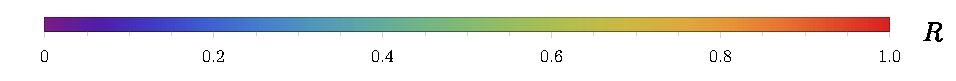
\includegraphics[width=\linewidth	]{0-RBar_h}\\
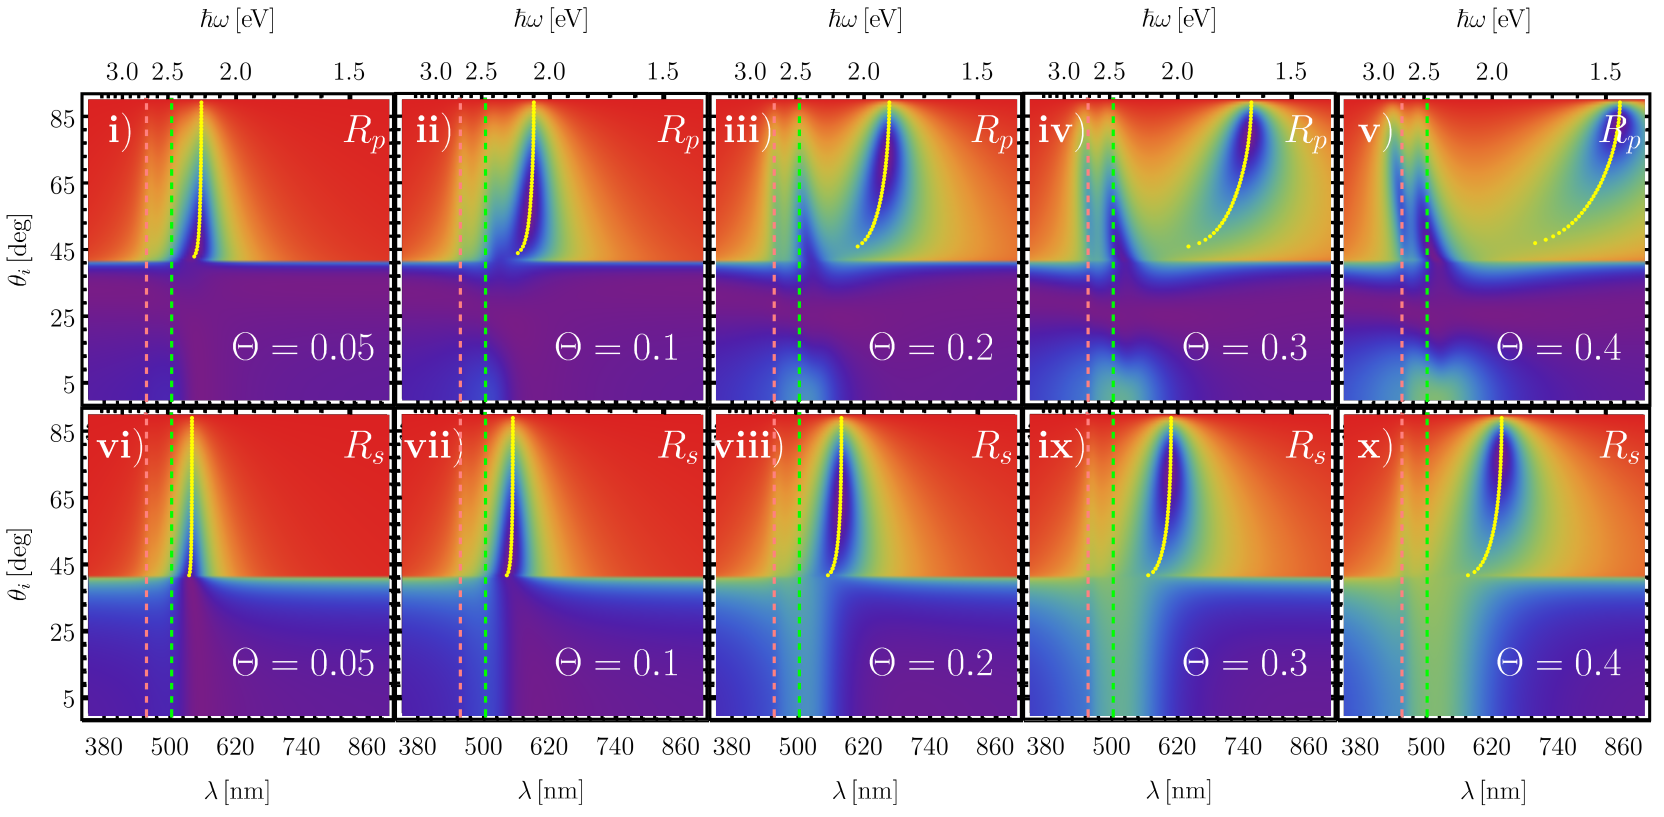
\includegraphics[width = .9\linewidth, trim={00 00 00 00}, clip	]{1-Wp4ThetaVar/0-2D_Grid}%
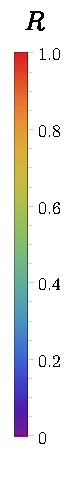
\includegraphics[scale=.85, trim={00 -5 00 00}, clip]{0-RBar_v}
	\caption{Gráficas de reflectancia de una monocapa en configuración ATR como función del ángulo de incidencia $\theta_i$ y de la longitud de onda $\lambda$ para una función dieléctrica tipo Drude con $\omega_p=4. 3$ eV  y  $\gamma=0. 15$ eV.  Las gráficas \{pol.  \emph{p} [$\mathbf{i)-v)}$] y pol.  \emph{s} [$\mathbf{vi)-x)}$]\} muestran los resultados para NPs de un radio de $a=30$ nm y distintas fracciones de cubierta $\Theta$: $0. 05$, $0. 1$, $0. 2$, $0. 3$ y $0. 4$. }	\label{fig:R-ATR4}	
	\end{figure}	
	

La reflexión de la luz en una interfaz plana entre dos medios es igual a la unidad para ángulos de incidencia mayores al ángulo crítico $\sin\theta_c = n_m/n_s$.  Para un sistema vidrio-aire $\theta_c\approx 41^\circ$.  En la Fig.  \ref{fig:R-ATR4} la refectancia para ángulos mayores al crítico es distinta de la unidad en regiones alejadas de las SPRs (líneas punteadas verticales) para partículas esféricas individuales, pues en dichas resonancias, la extinción de luz es máxima; Para fracciones de cubierta mayores, la extinción a las longitudes de onda de las SPRs es más evidente.  Adicionalmente al mínimo en $R$ debido a las SPRs, se presenta una región centrada en longitudes de onda mayores en donde la reflectancia es menor a la unidad.  Los puntos amarillos corresponden a mínimos anómalos en las mediciones de reflectancia para ángulos mayores al crítico y longitudes de onda mayores a la resonancia dipolar (línea vertical punteada verde).  La separación entre las longitudes de onda de las SPRs y los mínimos anómalos (puntos amarillos) aumenta conforme lo hace la fracción de cubierta $\Theta$; este comportamiento es más evidente en polarización \emph{p} que en \emph{s} [ver  Fig.  \ref{fig:R-ATR4} \textbf{v)} y \textbf{x}].  Dado que los puntos amarillos se localizan a longitudes de onda mayores ---equivalente a energías menores--- a la SPR dipolar, la excitación anómala no puede ser un modo de partícula individual, sino una respuesta colectiva como la SPLR. 

Para seguir estudiando el comportamiento anómalo en la reflectancia para una monocapa de NPs, se estudió una monocapa con NPs modeladas por el modelo de Drude-Sommerfeld con $\omega_p = 10$ eV pero manteniendo fijos los demás parámetros empleados en los resultados presentados en la Fig.  \ref{fig:R-ATR4}.  En la Fig.  \ref{fig:R-ATR10} se muestran los resultados de la reflectancia $R$ como función de la longitud de onda $\lambda$ y el ángulo de incidencia $\theta_i$, para el caso de una monocapa inmersa en vacío $n_m= 1$ y soportada por un sustrato de vidrio $n_s = 1. 5$.  La frecuencia de plasma empleada para la función dieléctrica de las NPs fue de $\omega_p = 10$ eV ($\lambda_p=123. 98$ nm) y una constante  fenomenológica $\gamma = 0. 15$ eV ($\gamma_\lambda=8,270$ nm); en la Fig.  \ref{sfig:Drude10eV} se muestra la gráficas la función dieléctrica y el índice de refracción con estos parámetros.  El radios de las NPs fue de $a=30$ nm y se calcularon los casos para las fracciones de cubierta $\Theta$: $0. 05$, $0. 1$, $0. 2$, $0. 3$ y $0. 4$, en polarización \emph{p} [en la Fig.  \ref{fig:R-ATR4}, $\mathbf{i)-v)}$] y en polarización \emph{s} [en la Fig.  \ref{fig:R-ATR4}, $\mathbf{vi)-x)}$].   El modo normal dipolar ($\ell=1$) corresponde a la línea vertical verde punteada en $\lambda \approx 502$ nm, y el modo cuadrupolar ($\ell=2$), a la línea vertical rosa punteada en $\lambda \approx 456$ nm. 
	
Al igual que en la Fig.  \ref{fig:R-ATR4}, la separación  entre el modo anómalo (puntos amarillos) y las longitudes de onda de las SPRs aumenta conforma lo hace la fracción de cubierta.  Asimismo, esta separación es mayor para la polarización \emph{p} que para la polarización \emph{s}.  Ya que el modo anómalo sufre un corrimiento al rojo para fracciones de cubierta mayores para las dos funciones dieléctricas empleadas,  se analizó si el comportamiento es semejante a cambios en el radio $a$ de las NPs.  Este analices se llevó a cabo ya que ambas cantidades modifican el volumen neto de material plasmónico.  De esta manera, se corrobora que los mínimos en anómalos $R$ se deben a un efecto colectivo de las NPs, al igual que las PSLR. 


	\begin{figure}[t!]\centering
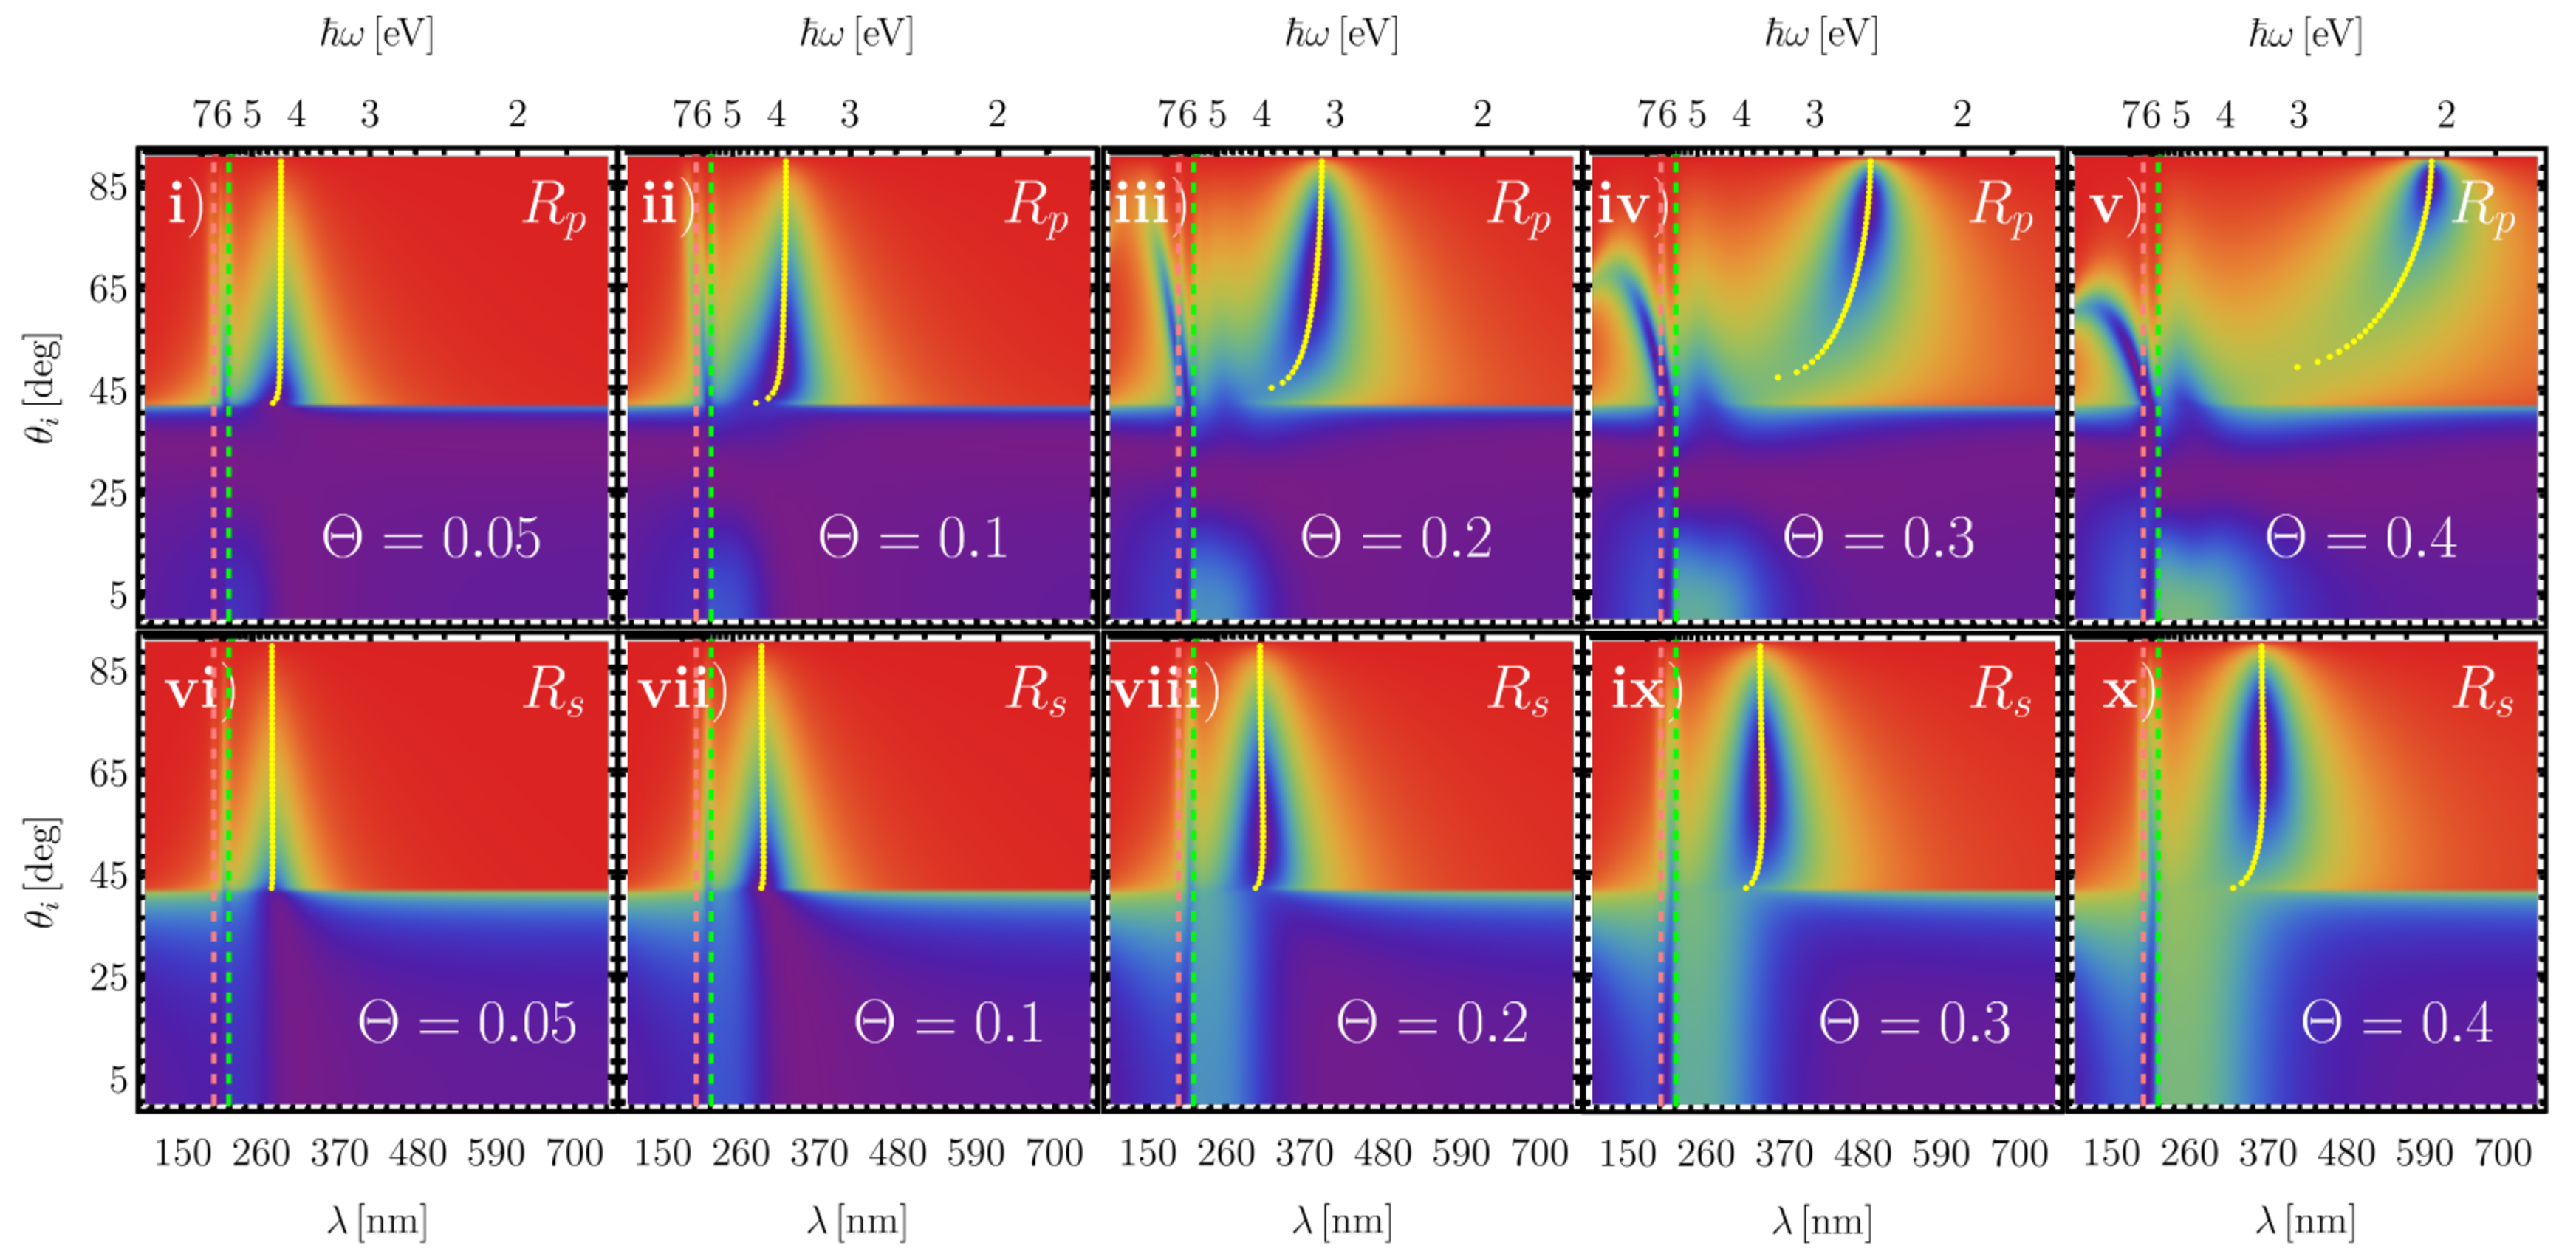
\includegraphics[width = .9\linewidth]{2-Wp10ThetaVar/0-2D_Grid}%
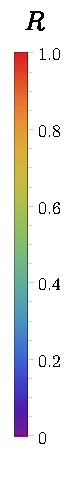
\includegraphics[scale=.85, trim={00 -5 00 00}, clip]{0-RBar_v}
	\caption{Gráficas de reflectancia de una monocapa en configuración ATR como función del ángulo de incidencia $\theta_i$ y de la longitud de onda $\lambda$ para una función dieléctrica tipo Drude con $\omega_p=10$ eV  y  $\gamma=0. 15$ eV.  Las gráficas \{pol.  \emph{p} [$\mathbf{i)-v)}$] y pol.  \emph{s} [$\mathbf{vi)-x)}$]\} muestran los resultados para NPs de un radio de $a=30$ nm y distintas fracciones de cubierta $\Theta$: $0. 05$, $0. 1$, $0. 2$, $0. 3$ y $0. 4$.  Los mínimos en la reflectancia ajenos a las SPRs se señalizan mediante los puntos amarillos. }	\label{fig:R-ATR10}	
	\end{figure}	

En la Fig.  \ref{fig:R-RVar} se muestran los resultados de reflectancia como función de la longitud de onda $\lambda$ y el ángulo de incidencia $\theta_i$ para una monocapa (con $\Theta=0. 3$) en configuración ATR inmersa en aire ($n_m=1$) y colocada sobre un sustrato con índice de refracción $n_s=1. 5$.  Los parámetros de la función tipo Drude empleada para simular a las NPs  en la Fig.  \ref{fig:R-RVar} son   $\omega_p = 4. 3$ eV ($\lambda_p=288. 5$ nm) y $\gamma = 0. 15$ eV ($\gamma_\lambda=8,270$ nm).  Se calcularon los casos para los radios $a$: $3$ nm, $5$ nm, $10$ nm y $20$ nm,  en polarización \emph{p} [en la Fig.  \ref{fig:R-RVar}, $\mathbf{i)-iv)}$] y en polarización \emph{s} [en la Fig.  \ref{fig:R-RVar}, $\mathbf{v)-viii)}$].  Las SPRs se corren hacia el rojo conforme aumenta el radio de las NP como se muestra en la Fig.  \ref{fig:NormalModes}. 

	\begin{figure}[b!]\centering
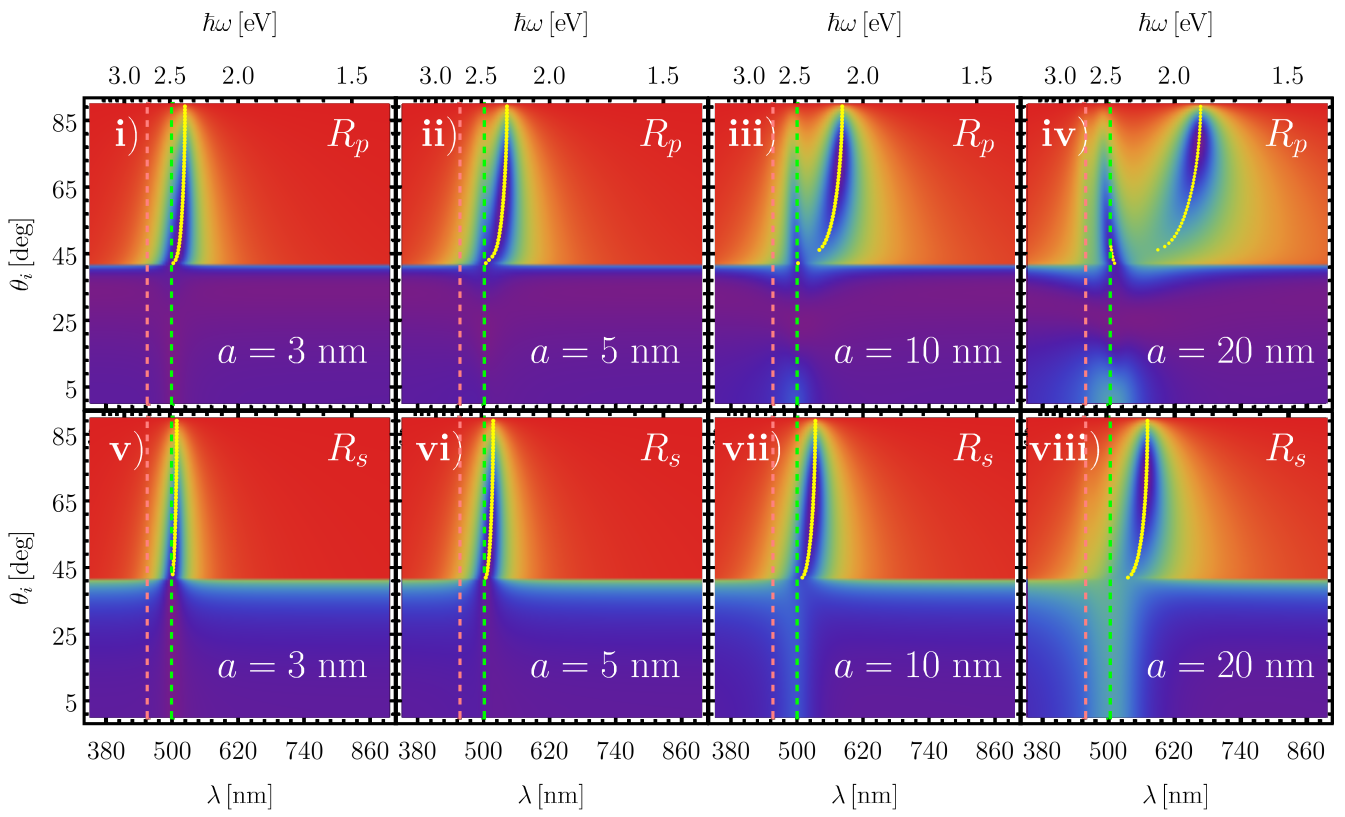
\includegraphics[width = .9\linewidth]{3-Wp4rVar/0-2D_Grid}%
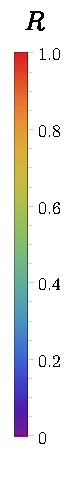
\includegraphics[scale=1, trim={00 -15 00 00}, clip]{0-RBar_v}
	\caption{Gráficas de reflectancia de una monocapa en configuración ATR ($\Theta = 0. 3$) como función del ángulo de incidencia $\theta_i$ y de la longitud de onda $\lambda$ para una función dieléctrica tipo Drude con $\omega_p=4. 3$ eV  y  $\gamma=0. 15$ eV.  Las gráficas \{pol.  \emph{p} [$\mathbf{i)-iv)}$] y pol.  \emph{s} [$\mathbf{v)-viii)}$]\} muestran los resultados para NPs de radio  $a$: $3$ nm, $5$ nm, $10$ nm y $20$ nm.  Los mínimos en la reflectancia ajenos a las SPRs se señalizan mediante los puntos amarillos. }	\label{fig:R-RVar}	
	\end{figure}	

La respuesta anómala de la reflectancia en la Fig.  \ref{fig:R-RVar} es señalada por los puntos amarillos.  La distancia estre ésta y las SPRs aumenta conforme crece el radio de las NPs $a$, al igual que lo hacía al incrementar la fracción de cubierta $\Theta$ en las Figs.   \ref{fig:R-ATR4} y \ref{fig:R-ATR10}.  De igual forma, se vuelve presentar una respuesta más evidente para la polarización \emph{p} que para la polarización \emph{s}.  Dado que los dos parámetros que modifican el número de electrones libres modifican la respuesta en reflectancia en zonas alejadas de las SPRs, se especula la existencia de un modo plasmónico semejante al PSLR reportado en  \cite{kabashin2009plasmonic} y \cite{danilov2018ultra}. 

Finalmente, se muestra en la Fig.  \ref{fig:R-JC} la respuesta óptica de una monocapa con fracción de llenado  $\Theta=0. 3$ y NPs de radio $a=30$ nm.  El índice de refracción del sustrato es $n_s=1. 5$ y el de la matriz $n_m=1$ sin embargo, la respuesta óptica de las NPs son los datos experimentales, obtenidos de \cite{johnson1972contants}, del Au [ver Fig.  \ref{sfig:JCAu}] y la Ag (ver \ref{sfig:JCAg}].  En la Fig.  \ref{sfig:JCAu} se presentan los resultados numéricos para el Au, para ambas polarizaciones y en la Fig.  \ref{sfig:JCAg} para la Ag. 

	\begin{figure}[h!]\centering
	\begin{subfigure}{.01\linewidth}\caption{}\label{sfig:JCAu}\vspace{4.5cm}\end{subfigure}\hspace*{-1em}
	\begin{subfigure}{.45\linewidth}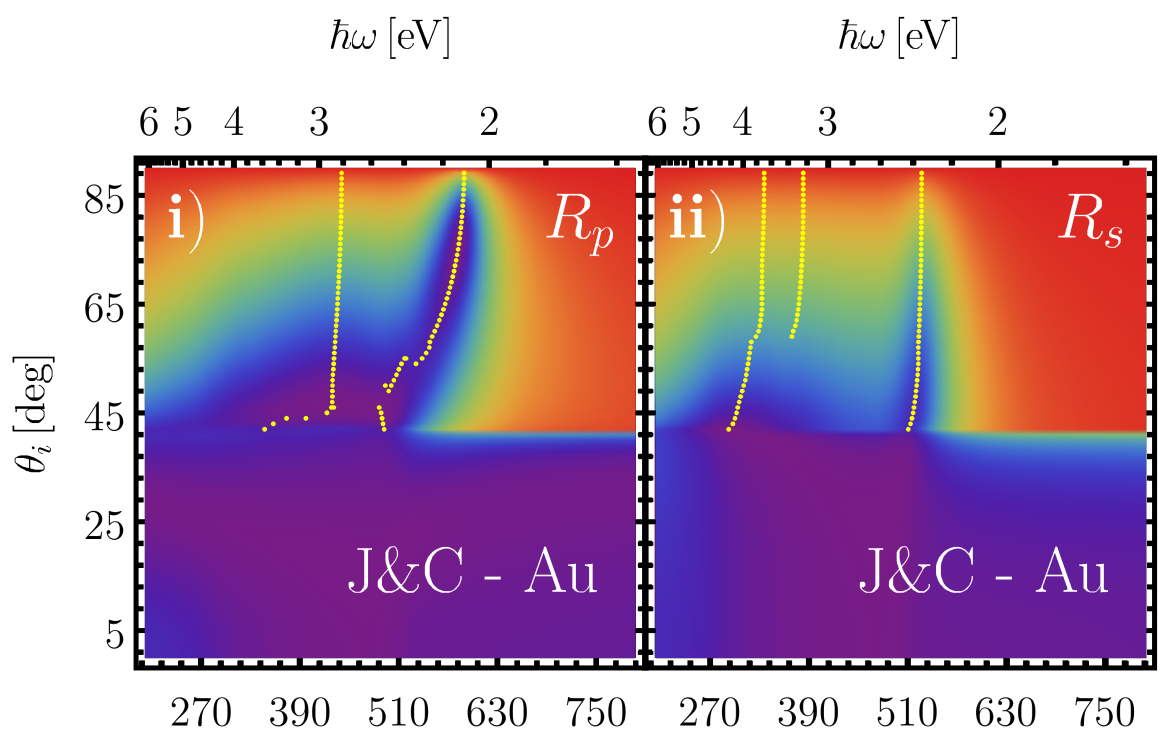
\includegraphics[width = .95\linewidth,]{5-JCAu/0-2D_Grid.png}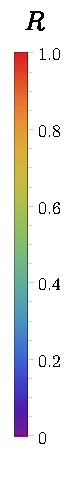
\includegraphics[scale=.6, trim={00 00 00 00}, clip]{0-RBar_v}
	\end{subfigure}
	\begin{subfigure}{.01\linewidth}\caption{}\label{sfig:JCAg}\vspace{2.5cm}\end{subfigure}\hspace*{-1.em}
	\begin{subfigure}{.45\linewidth}\centering 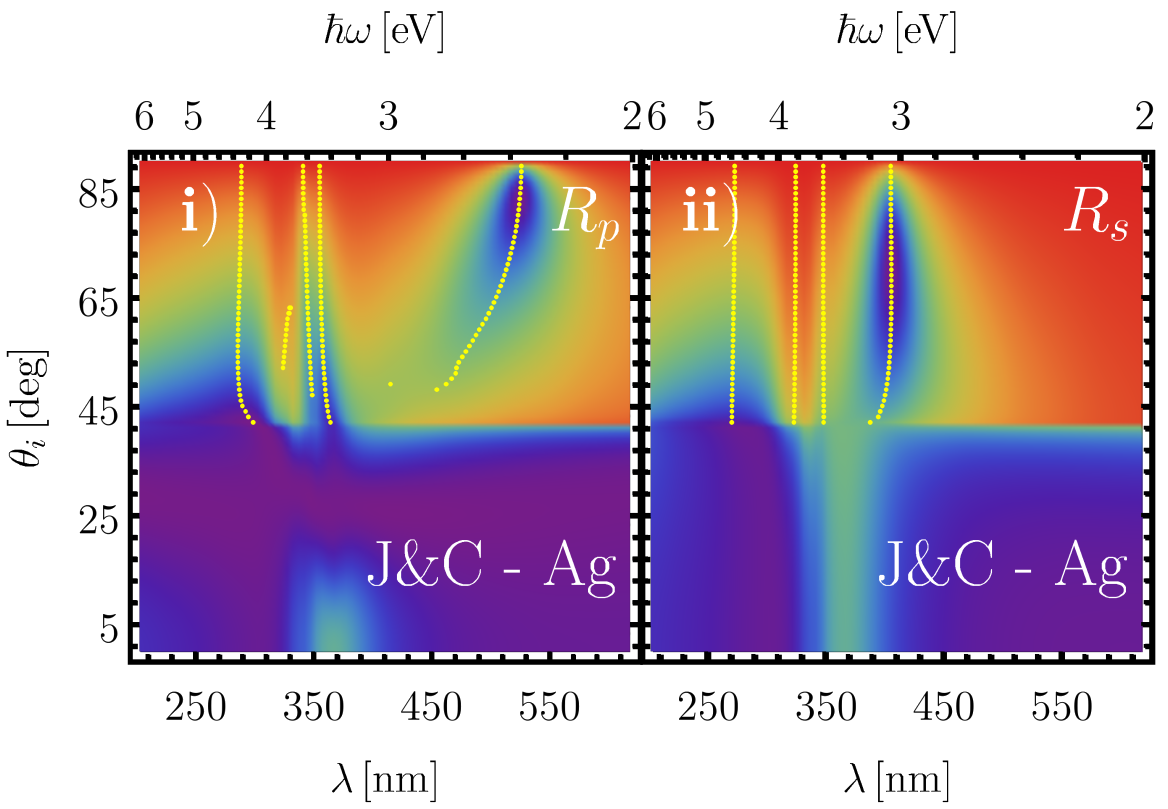
\includegraphics[width = .95\linewidth]{6-JCAg/0-2D_Grid.png}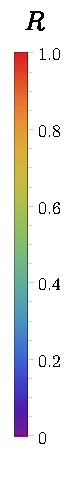
\includegraphics[scale=.6, trim={00 00 00 00}, clip]{0-RBar_v}\end{subfigure}
	\caption{Gráficas de reflectancia de una monocapa en configuración ATR ($\Theta = 0. 3$) como función del ángulo de incidencia $\theta_i$ y de la longitud de onda $\lambda$ para NPs de \textbf{a)} Au y \textbf{b)} Ag, calculados con los datos experimentales del índice de refracción tomados de \cite{johnson1972contants}.  Los mínimos en la reflectancia se señalizan mediante los puntos amarillos. }\label{fig:R-JC}
	\end{figure}	

En la Fig.  \ref{fig:R-JC} se representan en amarillo todos los mínimos en $R$ para distintos cortes en ángulos de incidencia.  En el caso del oro [Fig.  \ref{sfig:JCAu}] se presenta a $\theta_i=70^\circ$ la resonancia dipolar  a $438$ nm para polarización \emph{p} y a $379$ nm a polarización \emph{s}; la resonancia cuadrupolar no fue detectada para polarización \emph{p} mas a polarización \emph{s}  se localiza a $332$ nm.  El mínimo atípico en la reflexión se encuentra a $\theta_i=70^\circ$ en $576$ nm para polarización \emph{p} y a $524$ nm para polarización \emph{s}.  En el caso de la Ag [Fig.  \ref{sfig:JCAg}] se presenta a $\theta_i=70^\circ$ la resonancia dipolar  a $356$ nm para polarización \emph{p} y a $349$ nm a polarización \emph{s}; la resonancia cuadrupolar a $344$ nm en polarización \emph{p} y a $325$ nm en polarización \emph{s}.  El mínimo atípico en la reflexión se encuentra a $\theta_i=70^\circ$ en $523$ nm para polarización \emph{p} y a $406$ nm para polarización \emph{s}. 

%Para corroborar que el modo atípico es un modo guiado al igual que las SPLR, la transmitancia $T$ (Ec.  \eqref{eq:T}] no debe compensar las pérdidas de reflectancia a las longitudes de onda y ángulos de incidencia del modo atípico.  En la Fig.  \ref{fig:sum-JC} se muestra la suma de reflectancia y transmitancia (intensidad relativa medida $I/I_0$) para una monocapa de NPs esféricas de oro con un radio de $a = 9$ nm y una fracción de cubierta de $\Theta = 0. 3$ sobre un sustrato de vidrio ($n_s = 1. 5$) en una matriz de aire ($n_m = 1$).  El radio de la NP se escogió con la finalidad de despreciar los fenómenos de esparcimiento y sólo considerar la absorción del sistema.  Dado que la absorción ocurre al rededor de $300$ nm para NPs  el oro, al rededor de esta longitud de onda la intensidad relativa medida no puede ser igual a la unidad.  Por otro lado, en 
%
%	\begin{figure}[h!]\centering
%	\begin{subfigure}{.01\linewidth}\caption{}\label{sfig:sumJCp}\vspace{6. 5cm}\end{subfigure}\hspace*{-1em}
%	\begin{subfigure}{.41\linewidth}\centering 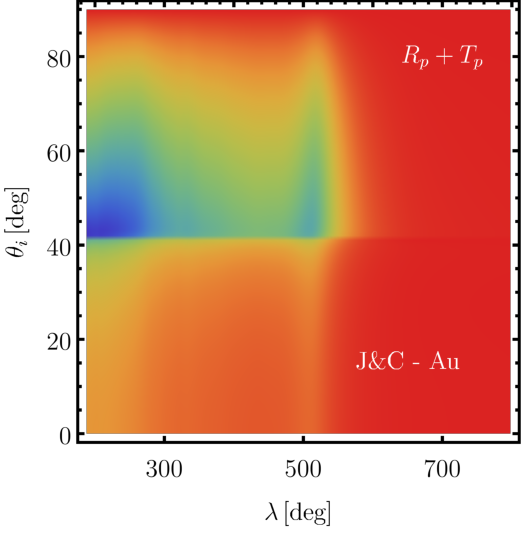
\includegraphics[scale=.8, trim={00 00 00 00}, clip]{5-JCAu/SUMp_4.pdf}\end{subfigure}
%	\begin{subfigure}{.01\linewidth}\caption{}\label{sfig:sumJCs}\vspace{6. 5cm}\end{subfigure}\hspace*{-1em}
%	\begin{subfigure}{.4\linewidth}\centering 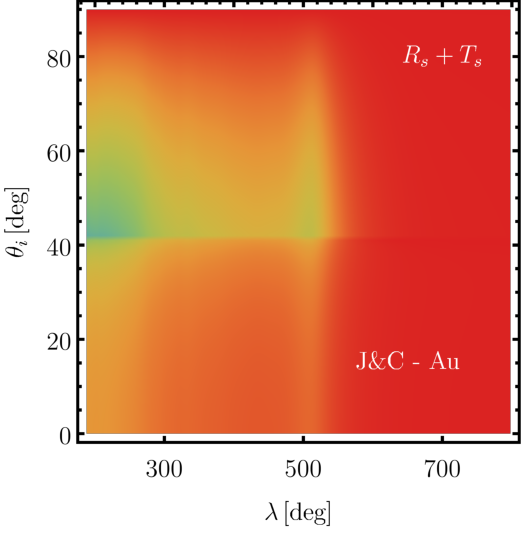
\includegraphics[scale=.8, trim={00 00 00 00}, clip]{5-JCAu/SUMs_4.pdf}\end{subfigure}
%	\begin{subfigure}{.1\linewidth}\centering 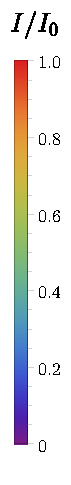
\includegraphics[scale=.9, trim={00 00 -10 00}, clip]{0-IBar_v}\end{subfigure}
%	\caption{Gráficas de la intensidad medida relativa $I/I_0$ de una monocapa en configuración ATR ($\Theta = 0. 3$) en polarización \textbf{a)} \emph{p} y \textbf{b)} \emph{s}, como función del ángulo de incidencia $\theta_i$ y de la longitud de onda $\lambda$ para NPs de oro y, calculados con los datos experimentales del índice de refracción tomados de \cite{johnson1972contants}. }\label{fig:sum-JC}
%	\end{figure}	

 \begin{thebibliography}{     }
 %
 \bibitem{boverhof2015comparative} D.  R.  Boverhof, C.  M.  Bramante, J. H.  Butala, S. F.  Clancy, M.  Lafranconi, J.  West, y S. C.  Gordon, ``Comparative assessment of nanomaterial definitions and safety evaluation considerations,'' \emph{Regul.  Toxicol.  Pharmacol. } \textbf{73}(1), 137--150 (2015). 
 %
\bibitem{zhao2008methods} J.  Zhao, A. O.  Pinchuk, J. M.  Mcmahon, S.  Li, L. K.  Ausman, A. L.  Atkinson, y G. C.  Schatz,``Methods for describing the electromagnetic properties of silver and gold nanoparticles,'' \emph{Accounts.  Chem.  Res. } \textbf{41}(12), 1710--1720 (2008). 
%
\bibitem{novotny2006principles} L.  Novotny, y B.  Hecht.  \emph{Principles of Nano-Optics} (Cambridge University Press, 2006). 
%
\bibitem{jain2008noble} P.  K.  Jain, X.  Huang, I.  H.  El-Sayed, y M.  A.  El-Sayed, ``Noble metals on the nanoscale: Optical and photothermal properties and some applications in imaging, sensing, biology, and medicine,'' \emph{Accounts.  Chem.  Res. } \textbf{41}(12), 1578--1586 (2008). 
%
\bibitem{stockman2011nanoplasmonics} M. I.  Stockman, ``Nanoplasmonics: The physics behind the applications,'' \emph{Phys.  Today} \textbf{64}(2), 39--44 (2011).  
%
\bibitem{bohren1998absorption} C.  F.  Bohren, y D. R.  Huffman,\emph{Absorption and scattering of light by small particles} (John Wiley \& Sons, 1998)
%
\bibitem{maier2007plasmonics} S.  A.  Maier, \emph{Plasmonics: fundamentals and applications} (Springer Science \& Business Media, 2007). 
%
\bibitem{kabashin2009plasmonic} A.  V.  Kabashin, P.  Evans, S.  Pastkovsky, W.  Hendren, G.  A.  Wurtz, R.  Atkinson, R.  Pollard, V.  A.  Podolskiy, y A.  V.  Zayats, ``Plasmonic nanorod metamaterials for biosensing,'' \emph{Nat.  Mater. } \textbf{8}(11), 867--871 (2009). 
%
\bibitem{danilov2018ultra} A.  Danilov, G.  Tselikov, F.  Wu, V.  G.  Kravets, I.  Ozerov, F.  Bedu, A.  N.  Grigorenko, y A.  V.  Kabashin, ``Ultra-narrow surface lattice resonances in plasmonic metamaterial arrays for biosensing applications,'' \emph{Biosens.  Bioelectron. } \textbf{104}, 102--112 (2018). 
%
\bibitem{atkinson2006anisotropic} R.  Atkinson, W.  R.  Hendren, G.  A.  Wurtz, W . Dickson, A. V.  Zayats, P.  Evans, y R.  J.  Pollard, ``Anisotropic optical properties of arrays of gold nanorods embedded in alumina,'' \emph{Phys.  Rev.  B} \textbf{73} (23), 235402 (2006). 
%
\bibitem{sihvola1999mixing} A.  H.  Sihvola, \emph{Electromagnetic mixing formulas and applications,} (Iet. , 1999). 
%
\bibitem{reyes2018analytical} A.  Reyes-Coronado,  A.  García-Valenzuela, O.  Z, and R.  G.  Barrera, ``Analytical modeling of optical reflectivity of random plasmonic nano-monolayers,'' \emph{Opt.  Express} 9594, 6697–6706 (2018). 
%
\bibitem{gross2014festkorperphysik} R.  Gross, y A.  Marx, \emph{Festkörperphysik} (Walter de Gruyter GmbH \& Co KG, 2014). 
%
\bibitem{griffiths2013electrodynamics} D. J.  Griffiths, \emph{Introduction to electrodynamics} (Pearson, 2013). 
%
\bibitem{truger2011properties} A.  Tr\"uger, \emph{Optical properties of metallic nanoparticles,} Diss.  Ph.  D.  thesis, Karl--Franzens--Universit\"at Granz, 2011. 
%
\bibitem{kreibig1995clusters} U.  Kreibig y M.  Vollmer.  \emph{Optical Properties of Metal Clusters} (Springer, 1995). 
%
\bibitem{ashcroft1976solid} N.  W.  Ashcroft, y N.  D.  Mermin \emph{Solid state physics} (Harcourt College Publishers, 1976). 
%
\bibitem{gauglitz2002handbook} G.  Gauglitz y D. S.  Moore \emph{Handbook of spectroscopy} (John Wiley \& Sons, 2014)
%
\bibitem{johnson1972contants} P.  B.  Johnson y R.  W.  Christy, ``Optical constants of the noble metals,'' \emph{Phys.  Rev.  B} \textbf{6}(12), 4370 (1972). 
%
\bibitem{mie1908metallosung} G.  Mie,  ``Beiträge zur Optik trüber Medien, speziell kolloidaler Metallösungen,'' \emph{Ann.  Phys. } \textbf{330}(3), 377–445 (1908). 
%
\bibitem{horvath2009historic} H.  Horvath, ``Gustav Mie and the scattering and absorption of light by particles: Historic developments and basics,'' \emph{J.  Quant.  Spectrosc.  Radiat.  Transf. } \textbf{110}(3), 787–799 (2009). 
%
\bibitem{arfken2001methods} G.  B.  Arfken, y  H.  J.  Weber, \emph{Mathematical methods for physicists} (Harcourt Academic Press, 2001)
%
\bibitem{maciel2017momentum} C.  A.  Maciel, \emph{Linear momentum transfer from swift electrons to small metallic nanoparticles: dipole approximation,} Diss.  Master thesis, Ms.  C.  thesis, Universidad Nacional Autónoma de México, 2017. 
%
\bibitem{aizpurua1998coupling} J.  Aizpurua, \emph{Coupling of electrons and electromagnetic surface modes in scanning transmission electron microscopy,} Diss.  Ph.  D.  thesis, Universidad de Pais Vasco, 1998. 
%
\bibitem{sihvola2007dielectric} A.  Sihvola, ``Dielectric polarization and particle shape effects,'' \emph{J.  Nanomater. } \textbf{1}, 1--9 (2007). 
%
\bibitem{pena-gomar2006coherent} M.  C.  Peña-Gomar, F.  Castillo, A.  García-Valenzuela, R.  G.  Barrera, y E.  Pérez, ``Coherent optical reflectance from a monolayer of large particles adsorbed on a glass surface,'' \emph{Appl.  Opt. } \textbf{45}, 626–632 (2006). 
%
\bibitem{garcia2012multiple} A.  Garc\'ia-Valenzuela, E.  Guti\'errez-Reyes, y R.  G.  Barrera, ``Multiple-scattering model for the coherent reflection and transmission of light from a disordered monolayer of particles,'' \textit{J.  Opt Soc.  Am.  A} \textbf{6}(29), 1161--1179 (2012). 
%
\bibitem{barrera2003coherent}  R.  G.  Barrera, y A.  García-Valenzuela, ``Coherent reflectance in a system of random Mie scatterers and its relation to the effective-medium approach,'' \emph{JOSA A}, \textbf{20}(2), 296–311 (2003).
%
\bibitem{svetovoy2008optical}  V. B. Svetovoy, P. J. Van Zwol, G. Palasantzas, y J. T. M. De Hosson, ``Optical properties of gold films and the Casimir force,'' \emph{Phys. Rev. B - Condens. Matter Mater. Phys.} \textbf{77}(3), 1–12 (2008).
% 
%\bibitem{ordal1985optical} M. A. Ordal, Robert J. Bell, R. W. Alexander, L. L. Long, y M. R. Querry, ``Optical properties of fourteen metals in the infrared and far infrared: Al, Co, Cu, Au, Fe, Pb, Mo, Ni, Pd, Pt, Ag, Ti, V, and W.,'' \emph{Appl. Opt.} \textbf{24}, 4493-4499 (1985)

\end{thebibliography}

\vspace{5cm}

\begin{center}
\begin{tabular} { c c }
\setlength{\tabcolsep}{15pt}
\renewcommand{\arraystretch}{1.5}
 \qquad \noindent\rule{6cm}{0.4pt}\qquad 		& \qquad \noindent\rule{6cm}{0.4pt}\qquad \\
 \qquad \textbf{Jonathan Alexis Urrutia Anguiano}  \qquad 		&    \qquad  \textbf{Dr.  Alejandro Reyes Coronado} \qquad \\
 \qquad Estudiante de la carrera de Física \qquad &  \qquad  Profesor Titular A de tiempo completo \qquad \\
\qquad No.  de cuenta: 414011025  \qquad 			& 	\qquad   Departamento de F\'isica, Facultad de Ciencias, UNAM \qquad \\
\qquad Tel. : +52 55 3110 1344 \qquad				& 	 \qquad Tel. : (55) 5622 4968\qquad \\
\qquad jaurrutia.95$@$ciencias.unam.mx	\qquad			&			\qquad  coronado$@$ciencias.unam.mx \qquad 
\end{tabular}
\end{center}


\end{document}

